%!TEX root = ../thesis.tex

\chapter{
  Illustrations of Human Movements
}
% Authoring Illustrations of Human Movements
% by Iterative Physical Demonstration

\newcommand{\systemname}{DemoDraw}
\newcommand{\phaseI}{Demonstration Interface}
\newcommand{\phaseII}{Refinement Interface}

Illustrations of human movements are used to communicate ideas and convey instructions in many domains, but creating them is time-consuming and requires skill.
We introduce a multimodal approach for people to generate these illustrations by physically demonstrating the movements.
Our \systemname{} system segments speech and 3D joint motion captured by a Kinect RGB-D sensor into a sequence of motion segments, each characterized by a key pose and salient joint trajectories.
Based on this sequence, a series of illustrations is automatically generated using a stylistically rendered 3D avatar annotated with arrows to convey movements.
During demonstration, users can also navigate existing illustrations using speech and amend or re-perform motions if needed. Once a suitable sequence of steps has been created, our system provides a \phaseII{} for finer control of visualization parameters.
In a three-part evaluation, we validate the effectiveness of the generated illustrations and the usability of both the \phaseI{} and the \phaseII{}.
Our results show that our participants could create 4-7 step-by-step illustrations from demonstrations in 22 minutes on average.

\begin{figure*}[t]
  \centering
  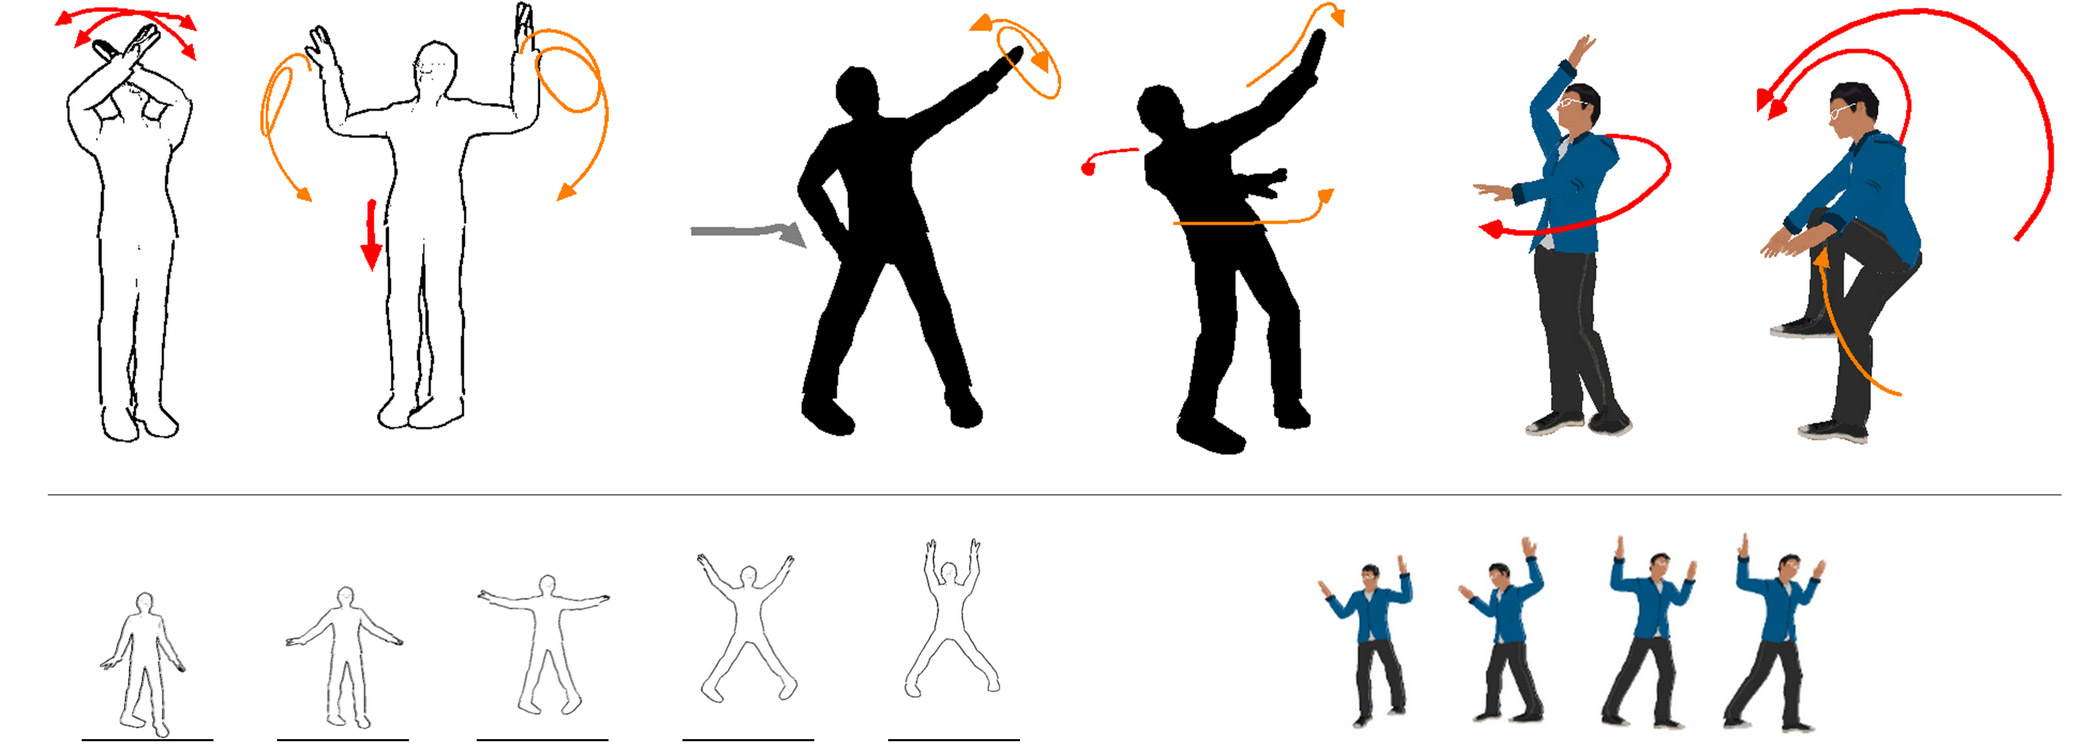
\includegraphics[width=\textwidth]{\demodraw/fig/teaser/teaser}
  \caption{\systemname{}: (a) multi-modal ``\phaseI{}'' to capture motion, verify results, and re-perform portions if needed; (b) conventional \phaseII{} for refinement and exploring other visualization styles; (c-d) examples of illustration styles.}
  \label{fig:demodraw_teaser}
\end{figure*}

%!TEX root = ../thesis.tex
\section{Introduction}

Popular online video-sharing websites such as YouTube have enabled the growth of a large community of users who share their knowledge and expertise in video tutorials. How-To videos demonstrate specific skills and procedures for tasks as varied as cooking, building a treehouse, or fixing a machine \cite{Torrey:2007he}.
These online tutorials help learners observe the manipulations and then put them into practice \cite{Torrey:2009fc}. However, in recording these videos, instructors often find it challenging to control the camera during demonstration.
%
Working with a cameraman who controls the device and viewpoints ensures that the video captures the movements that the audience would want to see, but it requires having a second person to direct the recording and work closely together with instructors. Many amateur users who mostly work alone, therefore, choose to self-record with one or more cameras. Camcorders can be set on a tripod to capture a static viewpoint, but it is hard to make sure whether users' actions are properly in frame at recording time. An alternative is to wear a head mounted camera to record what the instructors see. This may record unwanted and distractive head movements, making it difficult for the audience to watch. Additional camera views of the overall workspace might be needed to assist learners with understanding the context of demonstrated actions \cite{Fussell:2003te}.

\begin{figure}[t]
\centering
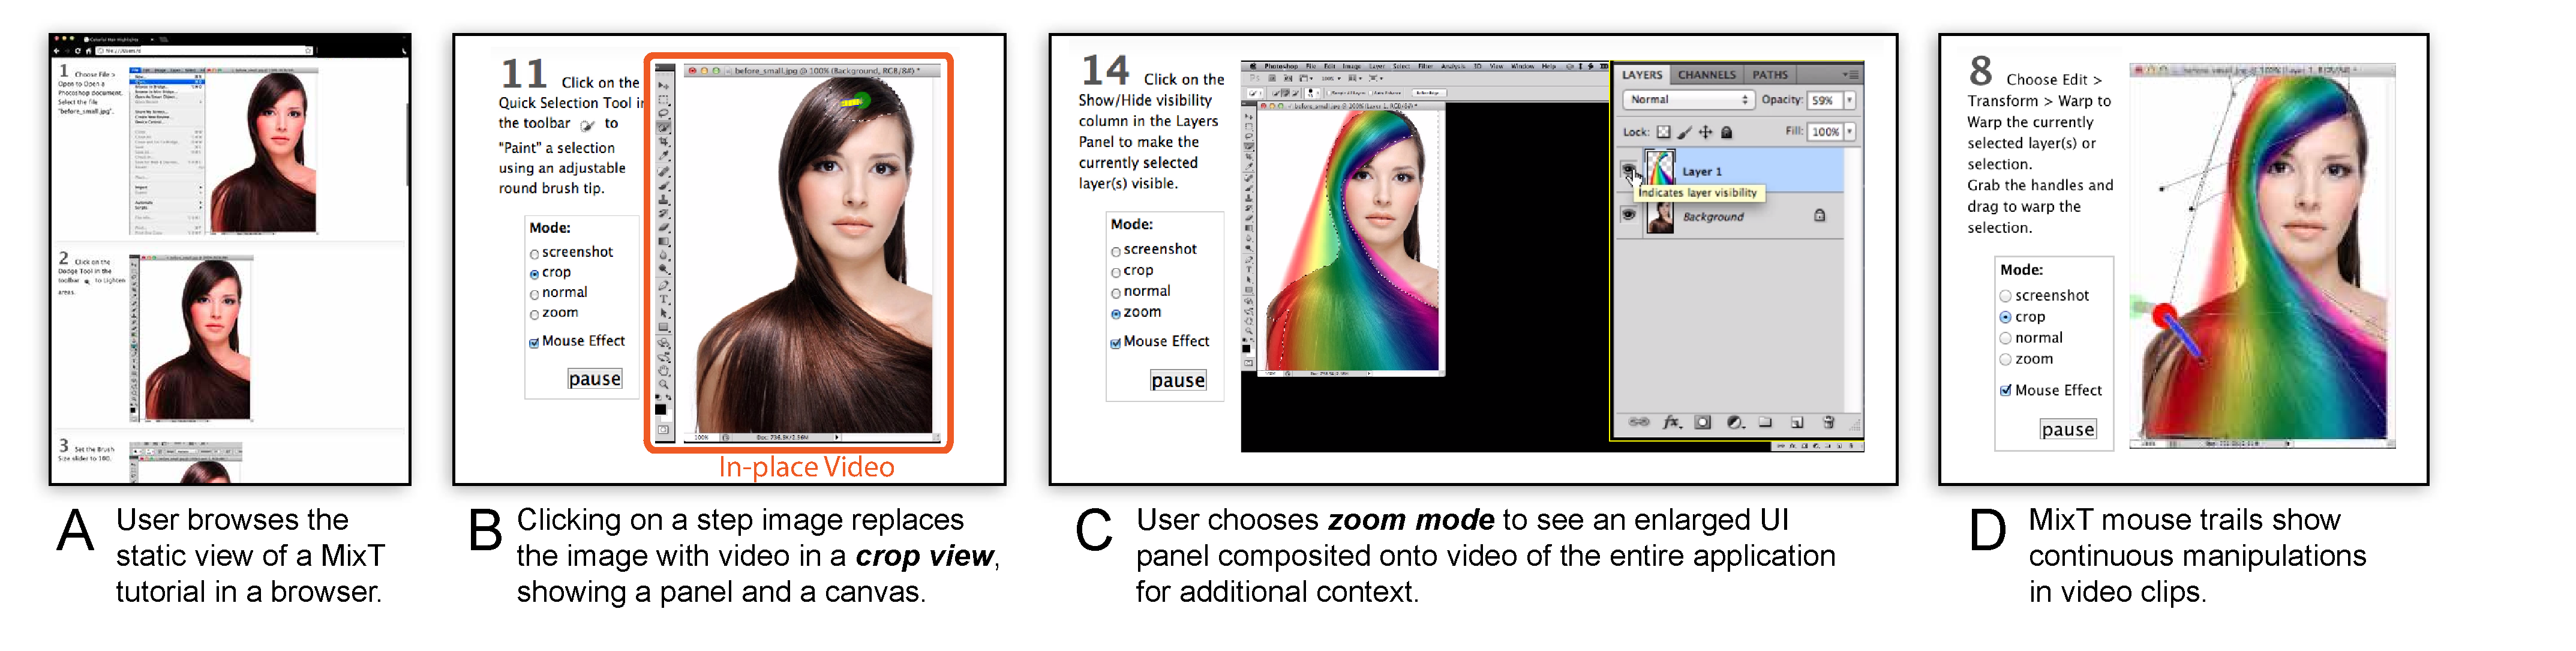
\includegraphics[width=0.8\columnwidth]{\kinectograph/fig/teaser.pdf}
\caption{Kinectograph includes a Kinect camera to track user movement and a motorized dock to pan and tilt the camera so that the user (or their hand) remains centered in the recorded video. Here the device follows the user\'s hand while he is illustrating.}
\label{fig:figure1}
\end{figure}

Seeing these filming challenges, we would like to enable users to gain the flexibility of real-time camera control without requiring a dedicated camera-person. Our goal is to design a device that can automatically track and orient to film the tutorial instructors while providing lightweight manual controls. Existing video conferencing cameras and surveillance tools offer human tracking to provide full or partial automatic viewpoint control. Polycom\footnote{http://www.polycom.com/} designs video conferencing cameras that feature face recognition and voice detection to enable a group of users to talk in an office room setting. This approach assumes people's faces should be in the frame, which may not be true for instructional videos that focus on actions rather than ``talking heads.''
%
Automatic motion tracking is possible to always keep the user in view using visible markers \cite{Ranjan:2010} or wearable sensors such as infrared emitters by Swivl\footnote{http://www.swivl.com/}. However, instructors are unlikely to take such approaches to put on visible markers when demonstrating.
%
Researchers have been developing techniques to track specific targets using computer vision, including hands \cite{Ranjan:2008}, user movements \cite{Wilson:2012fb}, fast-moving objects (e.g., a Ping-Pong ball) \cite{Okumura:2011tr}, or regions in pre-defined spaces \cite{Ranjan:2007}. These usually require an expert defining heuristics of space regions or movement classifications ahead of time for the tracking program. On the contrary, we aim at proposing a new approach that does not have these issues, gives users flexibility in a home environment, and provides interactive control over the behavior of the camera tracking.
%
% TeleAdvisor assists a helper to remotely observe a physical task in real-time and provide instructions~\cite{Gurevich:2012ko}. However, the system is limited by the static camera view without automatic tracking.
%

\clearpage
We propose Kinectograph, a new device that enables semi-automatic camera control for users to self-direct camera orientation for demonstration tasks (Figure~\ref{fig:figure1}). Kinectograph serves as both the camera and the cameraman. It provides a motorized dock for a Kinect\footnote{http://www.xbox.com/en-US/kinect} sensor and a tablet-based user interface (separate from the camera) to switch between tracking regions at runtime based on their needs when demonstrating. Using skeleton tracking to follow the user’s movement, Kinectograph automatically pans and tilts the camera in real time. Users can define zoom regions that follow his actions to provide closeup views. Using a Kinect sensor, our system works in a common indoor setting and does not require the user to wear sensors or configure the environments. Kinectograph makes a novel contribution over the prior art in its mixed-initiative approach that offers various levels of automation and control to users at record time.

In the following section (Section \ref{kinectograph_authoring}), we describe the user experience of recording with Kinectograph. We also describe design and implementation decisions (Section \ref{kinectograph_tracking}). Finally, in Section \ref{kinectograph_study}, we review findings from a preliminary evaluation with 7 participants to study Kinectograph's usability of self-recording tutorials. All of the participants successfully created a demonstration video using our system without assistance and found it easy to interact with.

%\bjoern{I cut this out because you are missing the reference.}\new{In [insert citation here], they similarly use motors and a camera to automatically track and zooming in on users, but they do so in a conference setting. One of their system objectives is to unobtrusively track; however, our system focuses on providing enabling user's control in these tracking and zooming decisions for their DIY tutorials. In addition they only use facial and audio tracking and do not leverage the power of the kinect to do skeletal tracking.}

% Abhishek Ranjan, Jeremy Birnholtz, Rorik Henrikson, Ravin Balakrishnan, Dana Lee. (2010). Automatic camera control using unobtrusive vision and audio tracking. Proceedings of GI 2010 – the Graphics Interface Conference. p. 47-54.
%\pc{Where is the reference to the papers Bjoern sent? auto-tracking camera}

%!TEX root = ../thesis.tex

\chapter{Related Work}
\label{chapter_related_work}

While existing practices require tutorial authors to create instructions manually, HCI and Computer Graphics communities have introduced novel technologies for authoring tutorials, including automatic generation methods and interactive editing tools.
%
In this chapter, I survey state-of-the-art techniques for generating instructions for both software applications (Section \ref{related_software}) and physical tasks (Section \ref{related_physical}).
%
Furthermore, existing instructions are mainly offered in the forms of conventional media, such as static tutorials (print-outs or web) or videos. With software systems, \keyword{interactive tutorials} have been introduced for learners to interactively review instructional content. I will discuss various forms of such kind of instructions by prior research, which leads to a discussion on the remaining gaps in tool support for creating and navigating instructional content.

% -------------------------------------------

\section{Instructions for Software Applications}
\label{related_software}

\subsection{Workflow Capturing and Tutorials}

Revealing operation history has shown to be effective in presenting software instructions. Operational events can range from low-level, application agnostic input device events (e.g., mouse actions, cursor movements, or keyboard strokes) to higher level, application-dependent information (e.g., menu selections or UI component changes).
%
Researchers have investigated automatic approaches that capture and visualize these types of events. Nakamura and Igarashi~\cite{Nakamura:2008:ASV:1449715.1449721} proposed a capturing and rendering system independent to GUI applications. Their system logs mouse events of a software demonstration process, including mouse moving, dragging, and clicking. Operations are rendered as markers and arrows on screenshot images to present the linear event history (see Figure~\ref{fig:related_events} top).
%
Grabler \ea{}'s approach~\cite{Grabler:2009jj} further analyzes the application context, including facial features and outdoor scenes, and annotates software screenshots with arrows, bounding boxes, and call-outs (see Figure~\ref{fig:related_events} bottom). In addition to annotated images, their system generates textual description from templates, such as \iquote{Select the \textbf{path tool} from the \textbf{toolbar} to \textbf{create and edit paths}.} The generated text and rendered images of operations are presented as a step-by-step tutorial, which is currently available as a Photoshop plug-in\footnote{Adobe labs. Tutorial Builder. \url{http://labs.adobe.com/technologies/tutorialbuilder/}}.

Demonstration-based approaches for generating instructions have been also applied to applications that involve more complicated manipulations or gestures, including 3D mesh construction~\cite{Denning:2011fy} and mobile apps~\cite{Wang:2014:EAC:2556288.2557407}.
%
Beyond logging events from recording a user demonstration, researchers have shown that workflows and software content can be captured automatically using application logs \cite{Grossman:2010jz,Grabler:2009jj,Pongnumkul:2011ju} or computer vision from analyzing desktop regions~\cite{Yeh:2009dh,Chang:2011vd} and existing screencast videos~\cite{Banovic:2012kd}.

\begin{figure*}[t!]
  \centering
  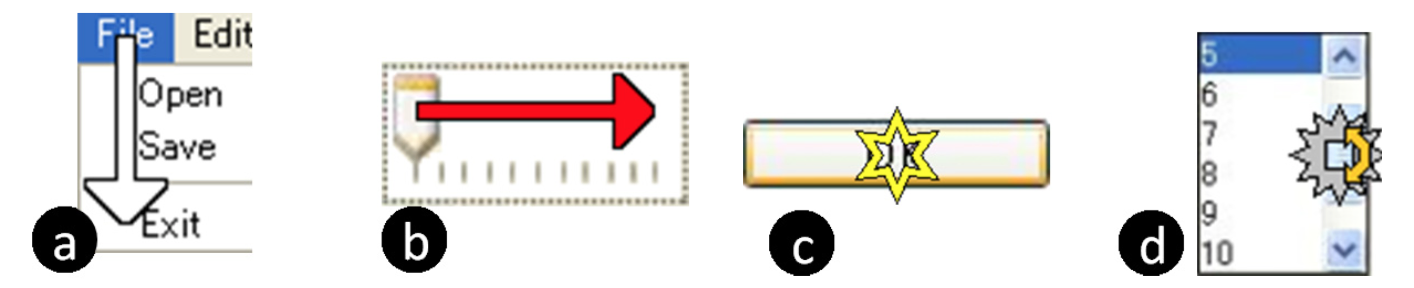
\includegraphics[width=0.6\textwidth]{\background/fig/software_viz/Nakamura_and_Igarashi}
  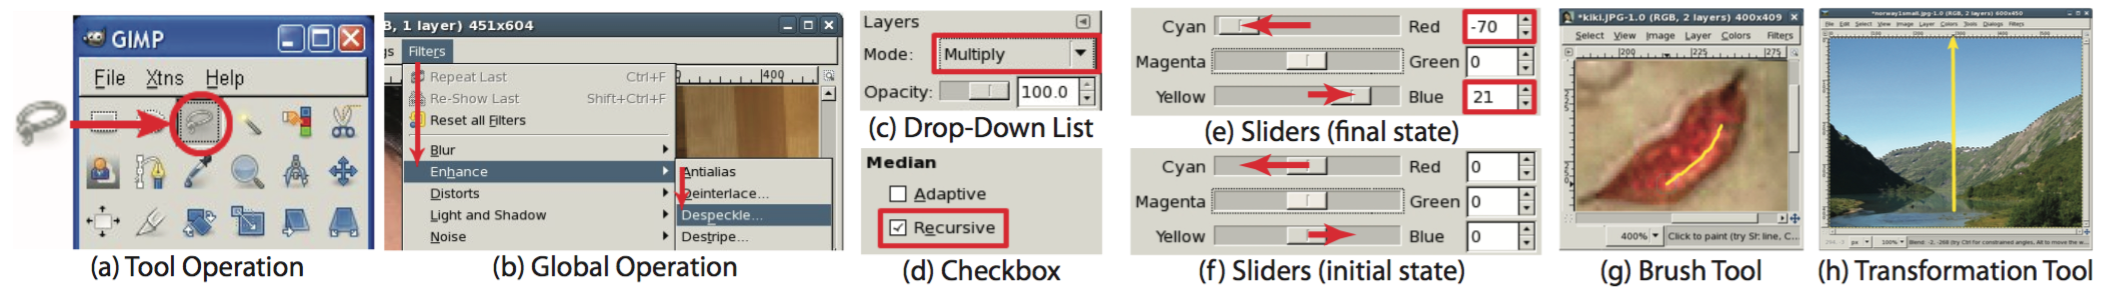
\includegraphics[width=\textwidth]{\background/fig/software_viz/Grabler}
  \caption{Example screenshots that visualize mouse operations are automatically rendered, including (top) mouse move, drag, click, and wheel (a-d) by Nakamura and Igarashi~\cite{Nakamura:2008:ASV:1449715.1449721} and (bottom) application-specific operations (a-b), parameters (c-f), and manipulations (g-h) by Grabler \ea{}~\cite{Grabler:2009jj}.}
  \label{fig:related_events}
\end{figure*}

To compare operation effects and workflows, other effective visualization approaches include showing a list of ``before'' and ``after'' thumbnails, video clips, and event timeline \cite{Grossman:2010jz} and creating a union graph of operations \cite{Kong:2012:DTR:2207676.2208549} (see Figure~\ref{fig:related_comparison}).

\begin{figure*}[t!]
  \centering
  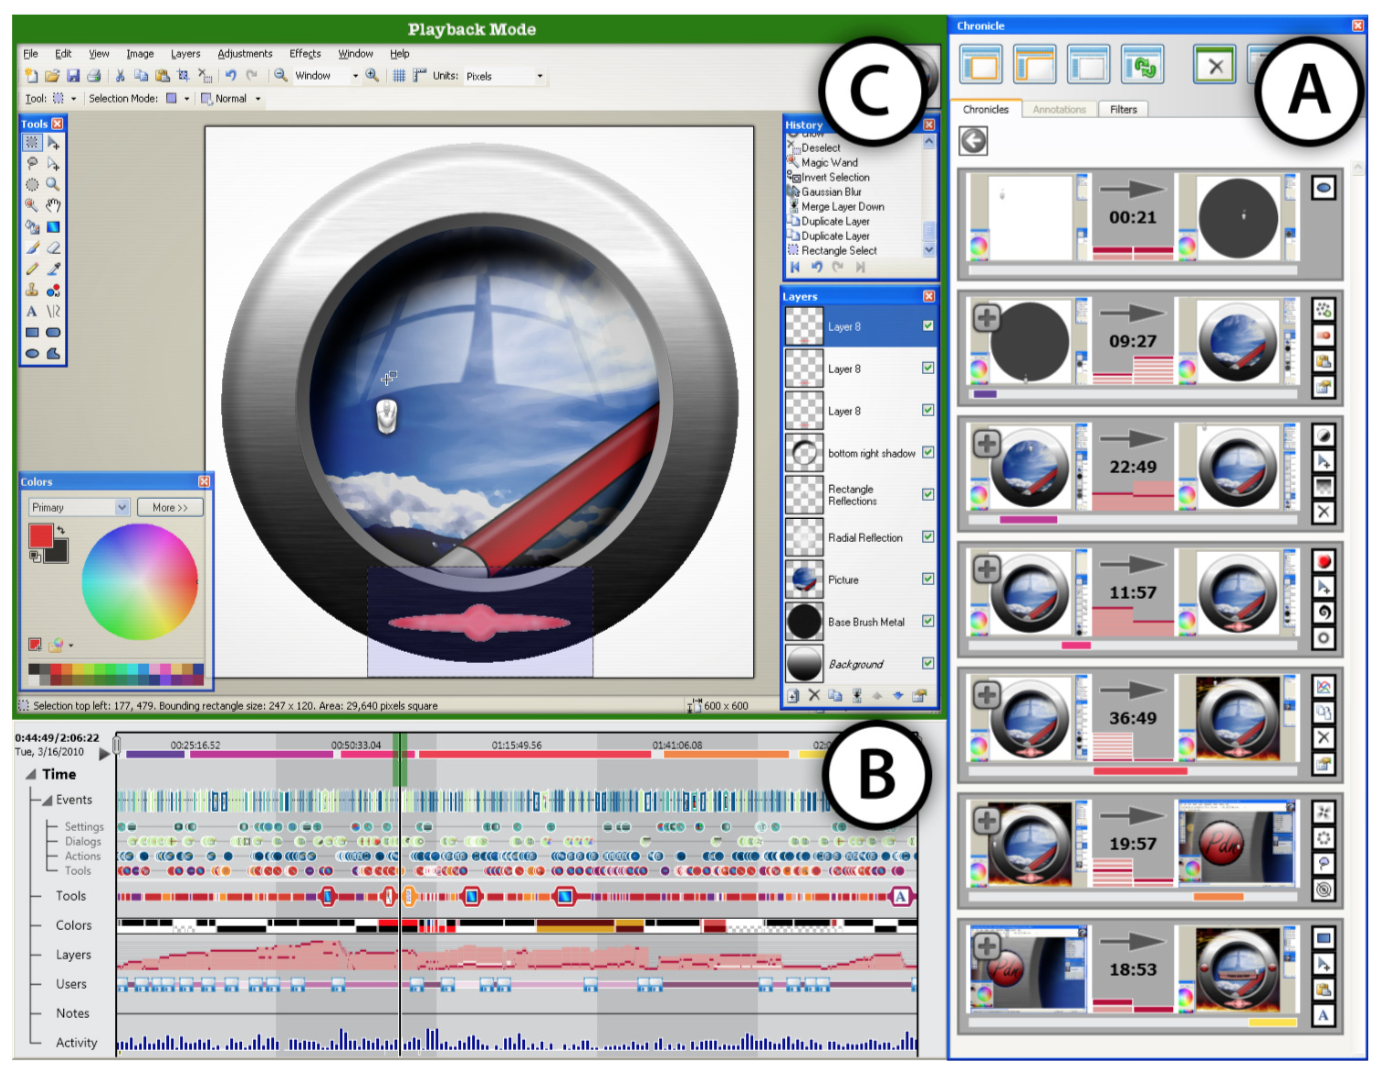
\includegraphics[width=0.4\textwidth]{\background/fig/software_viz/Grossman}
  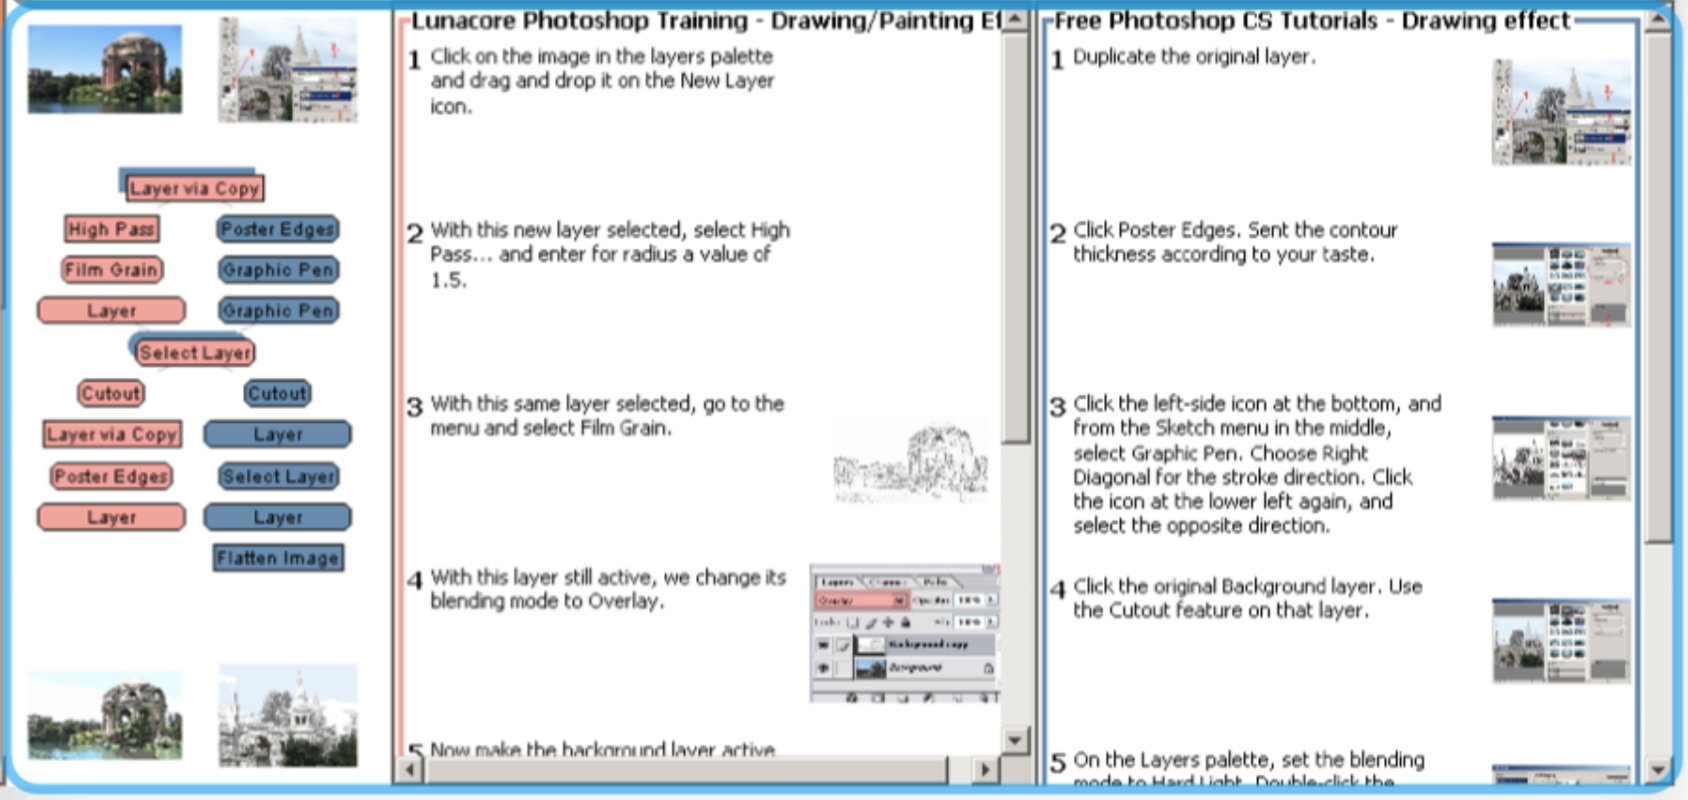
\includegraphics[width=0.55\textwidth]{\background/fig/software_viz/Kong}
  \caption{Instructional systems that help learners compare effects and similar tutorials using: (left) before and after images (a) and event timeline (b) by Grossman \ea{}~\cite{Grossman:2010jz} and (right) operation union graph by Kong \ea{}~\cite{Kong:2012:DTR:2207676.2208549}.}
  \label{fig:related_comparison}
\end{figure*}

% -------------------

\subsection{In-Application Support}

The above systems introduce innovative ways of providing informative screenshots or representations for learners to review workflows. However, reviewing these materials is often separated from operating a software application. Learners might have to switch between context of interacting an application and reading instructions, which could introduce a gap of evaluation (\iquote{Am I doing this right as the instructions explain?}) and a gap of execution (\iquote{How do I perform the action that the instructions describe?}).
%
Researchers have proposed another approach to provide ``in-application'' assistance, often in real-time, in a specific application context.

Studies have shown that visualizing input events in real-time during operations can provide better learnability of applications \cite{Dixon:2010fb}.
%
Commercial tools such as Mouseposé\footnote{Mouseposé \url{http://www.boinx.com/mousepose}} and ScreenFlow\footnote{ScreenFlow \url{http://www.telestream.net/screenflow}} visualize mouse and keyboard events with special effects, such as drawing a circle around a mouse cursor (see Figure~\ref{fig:related_realtime} top).
%
Dixon \ea{} proposed techniques to provide pixel-based enhancements in real-time, such as highlighting nearest regions of interest or applying afterglows based on the current user operations \cite{Dixon:2010fb,Dixon:2011:CHP:1978942.1979086} (see Figure~\ref{fig:related_realtime} bottom).

\begin{figure*}[t!]
  \centering
  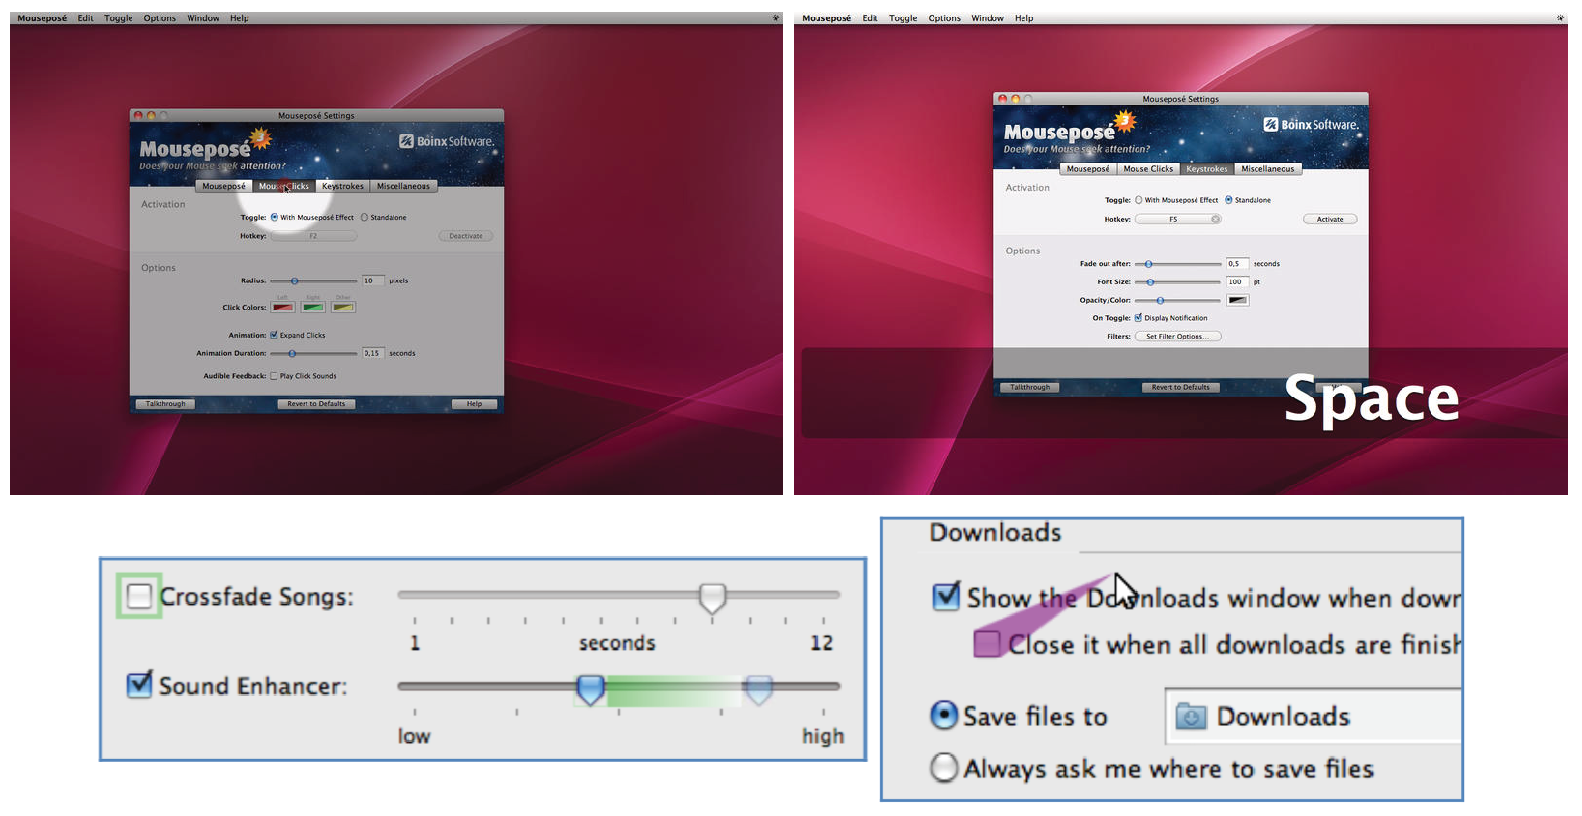
\includegraphics[width=0.7\textwidth]{\background/fig/realtime/realtime}
  \caption{Real-time visual enhancements on GUI applications: (top) Mouseposé highlights mouse cursors or text input; (bottom) Prefab creates target-aware or afterglow effects during user operating~\cite{Dixon:2010fb}.}
  \label{fig:related_realtime}
\end{figure*}

Real-time visual effects help users focus on the region of interest in a GUI application, but to support learners comprehend the application functionalities, there has been a considerable amount of research devoted to offering interactive helps.
%
Video snippets can be embedded in application tooltips~\cite{Grossman:2010wr}, which were shown to be seven times more effective than conventional tooltips for completing unfamiliar tasks.
%
Interactive, step-by-step instructions can be integrated in several forms:
%
To help user identify the correct UI components, tutorials can be shown via translucent colored ``stencils,'' which visually direct user's attention directly in an application~\cite{Kelleher:2005:STD:1054972.1055047}.
%
By tracking user's current operations, tutorials can be embedded in an application to provide instant feedback such as a check-mark or a percentage match~\cite{Fernquist:2011:SRE:2047196.2047245}, automatically replayed to provide the corresponding video instructions~\cite{Pongnumkul:2011ju}, or be shown as ambient help~\cite{Matejka:2011:AH:1978942.1979349}.
%
Instructions can be captured from demonstration as ``scripts'' for step-by-step navigation~\cite{Bergman:2005:DocWizards}. Having more user controls~\cite{Lieberman:2014:SML:2557500.2557543} or being enhanced with game elements~\cite{Li:2014:CGM:2556288.2556954, Dontcheva:2014:CCL:2556288.2557217} can further engage users in learning.

Last but not least, as tutorials are built for a broader community with a set of authors and learners, content can be dynamically updated within a community based on user contribution~\cite{Lafreniere:2013ff,Matejka:2009:CCR:1622176.1622214, Bunt:2014:TPI:2556288.2557118}.

interactive-visualization~\cite{Kwon:2016:CEO:2858036.2858101}
the paper that cited DemoWiz~\cite{Nguyen:2015:MST:2702123.2702209}

% These projects show how effective instructional representations can assist learners in learning or executing tasks. Our goal is to further study new formats that incorporate advantages of several formats of multimedia, including images, text, and videos, and in turn enhancing the learning experience for a variety of tasks.

% * define ``automatic''
% Note: MixT tutorials are automatically rendered from manual demonstration, not automatically generated.

% To provide real-time assistance, it is important to recognize the user activities during a task performance. Several domains have been widely studied, including software operations, scene recognition, and object tracking in a physical world.

% -------------------------------------------

\section{Instructions for Physical Activities}
\label{related_physical}

The above approach of tracking user behavior to automate tutorial authoring opens the door to interactive tutorials that can respond to user progress. However, tracking user behavior in the physical world, rather than in software, remains a challenge.

\subsection{Generating Instructions for Real-World Tasks}
Researchers have investigated tools for automatically generating visual instructions for physical tasks~\cite{feiner:1985:AEA:1299975.1300548,Seligmann:1991:AGI:127719.122732}. Workflows can be captured and created for furniture \cite{agrawala2003designing} or block assembly tasks \cite{Gupta:2012ku}.
%
If video content is difficult to be extracted, crowdsourcing algorithms have been introduced to structure step-by-step videos by online workers~\cite{Kim:2014:CSI:2611222.2556986}.
%
% New devices to support authors capturing multi-media materials, such as a turntable~\cite{Tseng:2015:SPT:2771839.2771869}
% documentation \cite{Tseng:2016:makeology}

\subsection{Interactive Guidance}
To provide responsive instructions, a computer system needs to understand user operations in real-time. Ideally, activities should be automatically tracked without human labeling.
%
Computer vision techniques can track specific physical targets, including hands \cite{Ranjan:2008}, user movements \cite{Wilson:2012fb}, fast-moving objects (e.g., a Ping-Pong ball) \cite{Okumura:2011tr}, or regions in pre-defined spaces \cite{Ranjan:2007}.
%
These methods usually require an expert defining heuristics of space regions or movement classifications ahead of time for the tracking program.
%
Thanks to the advance of technology, camera sensors such as Kinect have become widely available to track activities for block assembly~\cite{Gupta:2012ku} and dance~\cite{Anderson:2013:YEM:2501988.2502045}.

Real-time guidance is often shown via an external display, placed next to the working area~\cite{Gupta:2012ku}. To better blend the information into activities, Knibbe~\ea{} design a display-embedded table as a physical workspace that monitors, records, and assists users~\cite{Knibbe:2015:SMI:2817721.2817741}.
%
Alternatively, information can be overlaid on top of the work area using augmented reality, usually through a head-mounted display. Such systems can provide visual highlights for machine maintenance~\cite{Henderson:2011ff}, or interactive remote tutoring for repair tasks~\cite{Gurevich:2012ko}.
%
Another method is to overlay guidance on an augmented mirror for tasks such as dance movements~\cite{Anderson:2013:YEM:2501988.2502045}.

for Frisbee players~\cite{Solomon:2014:UTI:2540930.2540965}

% Lovell and Buechley use electrical sensing with conductive thread for a sewing tutorial~\cite{Lovell:2010tl}.

% I aim to propose a new approach that gives users flexibility in a home environment, and provides interactive control. If activity recognition is not possible, my approach includes users in the loop to annotate high-level information in order to create high-quality results.

% -------------------------------------------

\section{Working with Videos}

\tofix{intro here}

\subsection{Capture}
Several research and commercial systems guide users at capture time to yield higher-quality videos. Such systems often employ templates to help users capture sequences of distinct shots (e.g., Snapguide\footnote{\url{http://snapguide.com/}}) or suggest framing of the subject or camera view as in NudgeCam~\cite{Carter:2010}. Computer vision algorithms, like face tracking, can be used to offer real-time feedback during such directed actions~\cite{Davis:2003cu,Heer:2004ba,Carter:2010}. Instead of relying on templates, shot suggestions can also be bootstrapped through user dialogs~\cite{Adams:2005}.

\subsection{Annotation}
Researchers have investigated how to provide interactions that enable efficient, fluid annotation of video data, from the early EVA system~\cite{Mackay:1989} to more recent interfaces like VideoTater that leverage pen input~\cite{Diakopoulos:2006vt}.

\subsection{Editing}
Frame-based editing of video is very time-intensive, as it forces users to operate at a very low level of detail. Editors can leverage metadata, such as transcripts~\cite{Berthouzoz:2012,Pavel:2014:VDB:2642918.2647400} and shot boundaries~\cite{Casares:2002dx}, to give users higher-level editing operations at the shot level rather than the frame level.
In specific video domains like interview videos, transcripts can help users place cuts and transitions~\cite{Berthouzoz:2012}.
%
Computer vision techniques can automate certain effects, such as creating cinemagraphs~\cite{Bai:2012, Joshi:2012}, automatically-edited lecture videos~\cite{Heck:2007}, zoomable tapestries~\cite{Barnes:2010} and synopses~\cite{Pritch:2009vl}, or stabilizing shaky amateur videos~\cite{Liu:2011}. When analyzing video is a matter of subjective taste, identifying salient frames can also be outsourced to crowd workers~\cite{Bernstein:2011uj}.

live authoring through compositing and editing of streaming video~\cite{Freeman:2014:LLA:2611105.2557304}

\subsection{Navigating}
Videos can be navigated at the content level beyond log events, such as visualizing subject movements in a storyboard design \cite{goldman2006schematic} and enabling direct manipulation of a target in 2D \cite{Dragicevic:2008:VBD:1357054.1357096,Goldman:2008:VOA:1449715.1449719,Karrer:2008:DDM:1357054.1357097} or 3D \cite{Nguyen:2013:DMV:2470654.2466150}. These techniques help viewers understand content flow and playback videos, and have been applied to screencast videos \cite{Denoue:2013:RDM:2451176.2451190}. It is also possible to automate video control based on user actions for scenarios such as operating software applications~\cite{Pongnumkul:2011ju} and block assembling tasks \cite{Gupta:2012ku}. Such novel forms of video navigation inspired us to explore new visual designs for revealing the video content that support live presentations.

lecture videos~\cite{Tang:2006:DIU:1111449.1111523}

Visualization of personal history for video navigation~\cite{Al-Hajri:2014:VPH:2611105.2557106}

% In contrast to these systems, we do not require the author to manipulate the camera or system during capture. Many leisure activities, such as home repair or cooking, require use of both hands or involve getting one's hands dirty, so camera manipulation is not possible. We use vision techniques for automatic recording and editing. It differs from previous approaches in its focus on particular application domains -- software and physical demonstrations. By focusing on specific domains, we can make assumptions about the structure of the input and output video, such as the fact that there is a linear set of steps or movements, and offer user interfaces and algorithms that make it easier to create high quality instructions.

%!TEX root = ../thesis.tex
\section{Design Guidelines}

Researchers provide different findings on the effectiveness of media formats of software tutorials. Evaluating the instructional potential of videos began in the 1990s. Palmiter, Elkerton [16,17], and Harrison [11] studied the effect of animated demonstrations on learning and instruction recall. More recently, Grabler et al. compared how users followed book tutorials, videos, and automatically generated static tutorials [8]. Their results showed that automatically generated text and image tutorials outperformed video or book instructions on time and errors. Grossman et al. studied the effectiveness of embedding short (10-25 second) video clips in applications [9]. They found that participants who had access to video-based tooltips were significantly faster in completing tasks than those who viewed static ones.

While these studies suggest that there is still some debate over the tradeoffs between step-by-step static and video tutorials, they provide strong support for two key claims: step-by-step tutorials help users make fewer errors by allowing them to work at their own pace, while videos can help provide subtle details of complex interactions that are difficult to represent statically. Based on these findings, we designed a formative user study that investigates whether video clips can be incorporated into a step-by-step framework to help users follow certain types of image-editing tasks within a tutorial.

\subsection{Formative User Study}

\begin{figure*}[t]
  \centering
  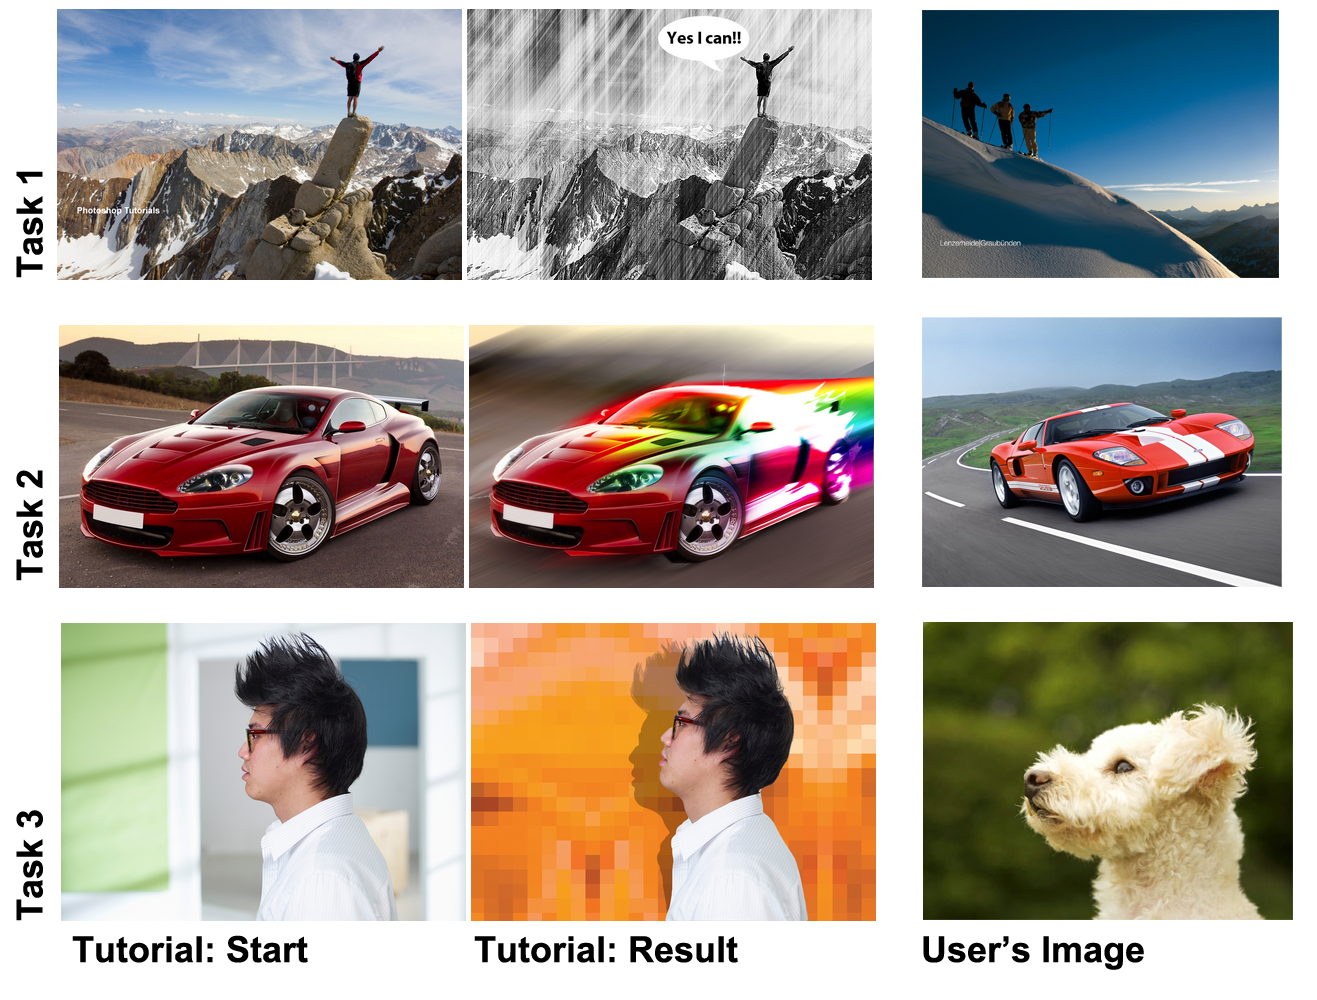
\includegraphics[width=\textwidth]{\mixt/fig/formative_study/study-images}
  \caption{In our formative study, participants completed three tutorials with images similar but not identical to the originals.}
  \label{fig:formative_tasks}
\end{figure*}

\begin{figure*}[t]
  \centering
  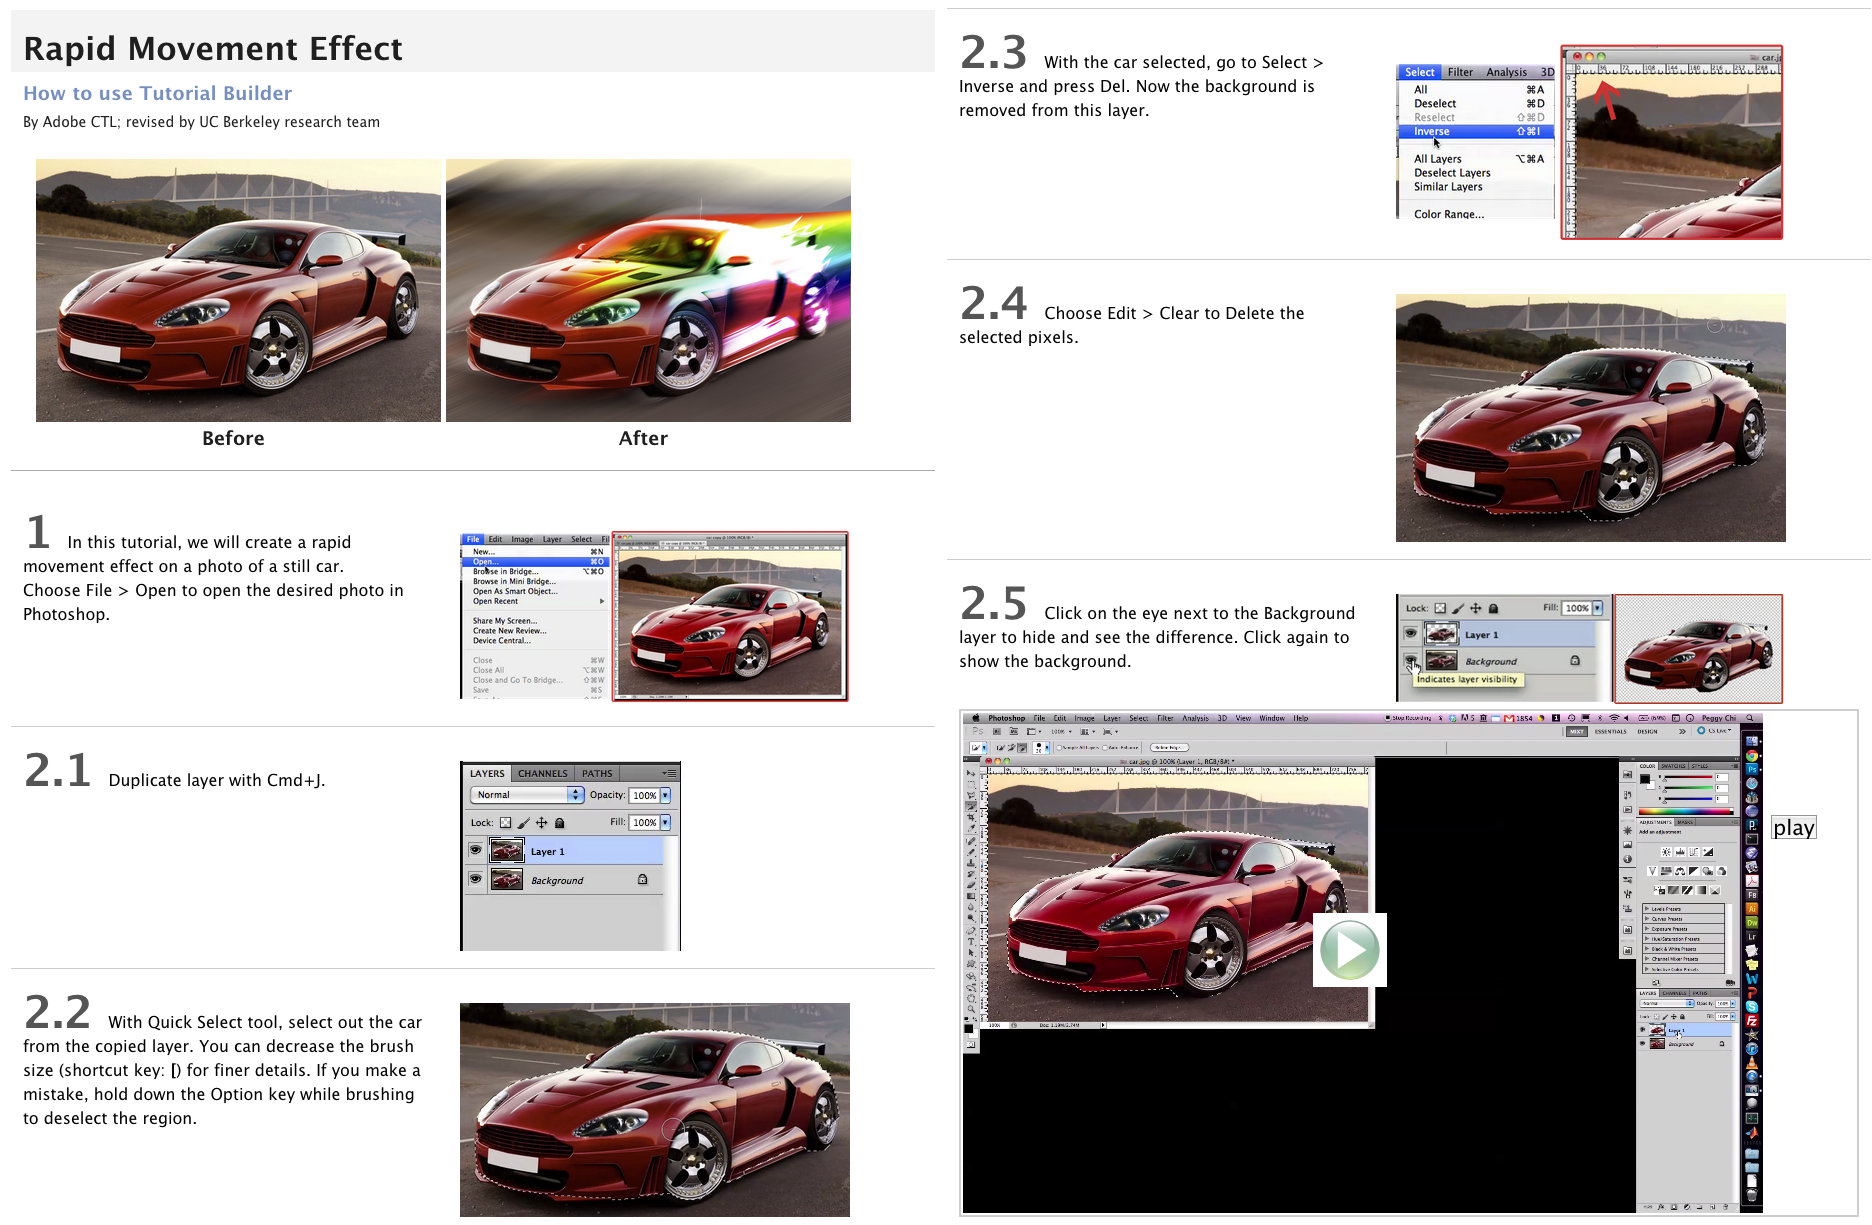
\includegraphics[width=\textwidth]{\mixt/fig/formative_study/study-mixed-example}
  \caption{In the mixed condition, participants saw an HTML page with static images and text; they could expand each step to view a video of that step (here: step 2.5).}
  \label{fig:formative_mixt}
\end{figure*}

% \subsubsection{Study Design}
\subsubsection{Hypothesis}
Our formative study aims to test the following two hypotheses:

H1: Image manipulation tutorials that mix static images and video clips are more effective than all-static or all-video tutorials.

H2: Users benefit more from seeing video clips instead of static text and images for certain types of commands.

\subsubsection{Participants}
We recruited 12 participants (5 males and 7 females, aged 20-52), 4 from a campus student design group and 8 from a computer software company, and compensated each with a \$15 gift card for participating. Our tutorials focused on achieving specific tasks in Adobe Photoshop. We recruited participants who had prior expertise with Adobe Photoshop, but who were not expert users. To demonstrate expertise, potential participants first completed an online screening test that asked them to follow a short image manipulation tutorial and submit the resulting file. The selected participants had between 1 and 20 years of experience using Photoshop.

\subsubsection{Tasks and Material}
The study was based on a within-subject design. We looked through Photoshop books and selected 3 different image manipulation tasks with similar levels of difficulty and complexity (see Figure~\ref{fig:formative_tasks}). Each tutorial comprised 15-20 steps. We focused on tutorials that included new, less common features such as the liquify tool, gradient warp tool, and puppet warp tool to increase the chance that participants would encounter unfamiliar tools. For each tutorial, we created three types of presentations: 1) static (in HTML format displayed on the screen), 2) video (on YouTube with audio narration), and 3) mixed (web interface shown in Figure~\ref{fig:formative_mixt} without audio). To ensure that different formats presented equivalent information where possible, we first recorded and narrated our video tutorials, then manually generated the static version by writing text instructions based on the narration and annotating and cropping frames of the video. To create mixed tutorials we started with the static tutorials and added the corresponding screencapture video segment for each step. To view the video segment for a step in the mixed tutorial, the user had to click on the image for that step. We scaled these videos to a fixed resolution of 800x500 pixels so that at least 2-3 steps would fit on screen when the videos were expanded. Many online tutorials do not offer full-screen resolution videos; even when high-resolution videos are available, they are hard to use as they force users to continually switch between the video and application windows. We disabled the soundtrack in the mixed tutorial to avoid situations when users only relied on auditory instructions instead of learning from static or video formats.

For each task, participants were given a source image that was distinct, but thematically similar to the image manipulated in the tutorial itself. This study design choice was motivated by the fact that users typically want to transfer the techniques found in tutorials to their own images.

\subsubsection{Procedure and Environment}
Each session consisted of 1 warm-up task and 3 experimental tasks. The warm-up task was a short 5-step static tutorial. In the 3 experimental tasks the format and task order were randomized. Each 60-minute session was conducted in a lab environment, using computers running Mac OS X, Adobe Photoshop CS5.1 and a web browser (Google Chrome) for viewing tutorials. Each participant was provided with a keyboard and a mouse and was allowed to adjust the equipment setting such as the monitor position and mouse tracking speed during the warm-up task. Photoshop and the web browser were arranged side-by-side on a 30-inch monitor with a resolution of 2048x1280 pixels. During the study, we used screen capture software to record user performance.

\subsubsection{Measurement}
To evaluate H1, we report the number of errors and repeated attempts that the participants made for each task. While our ultimate goal is skill acquisition and retention, we focus on the pragmatic goal of improving users' success in following tutorials and performing the instructions. We record an error if the participant performed a command incorrectly or skipped a step in the tutorial. While errors give a sense for the effectiveness of the tutorials, they do not measure the extraneous work users might have to perform when they have trouble understanding the correct outcome of a step. For example, if a user makes an error and then correctly executes several steps before recognizing the problem, we count this as a single error, even though the user must go back to fix the problem and then redo the subsequent steps. In addition, users may select the right command, but be dissatisfied with the result of their image and try again (e.g., redrawing a gradient). In such cases, we record all executions of the same step following the first attempt as a repeated attempt. Note that we do not count adjustments of continuous parameters or refinements of selection regions as repeated attempts because in these cases, the user is focusing on a single action rather than repeating a previously executed step. We do count a repeated attempt if the user entirely undoes a step to then retry it.

To evaluate H2, we count the number of different users who click on the video for each step in the mixed tutorials. To determine whether some types of commands benefit from videos more than others, we bin each step into one of the following five command categories based on the types of user interaction and UI elements it involves: brushing/drawing, manipulating control points (e.g., mesh-based warping, spline editing), parameter adjustment (e.g. using a slider to change opacity), UI navigation (e.g., switching tools, finding menu items), and layer operations.

We also collect qualitative data by observing how users follow the presented information and obtain additional feedback via 5-point Likert-scale questions (e.g., “The {\textless}condition{\textgreater} tutorial was easy to follow.”) and open-ended questions (e.g., “Compared with static tutorials, what were the pros and cons of the mixed media tutorial?”).

%!TEX root = thesis.tex
% User scenario using the DemoDraw system

\begin{figure*}[!t]
  \centering
  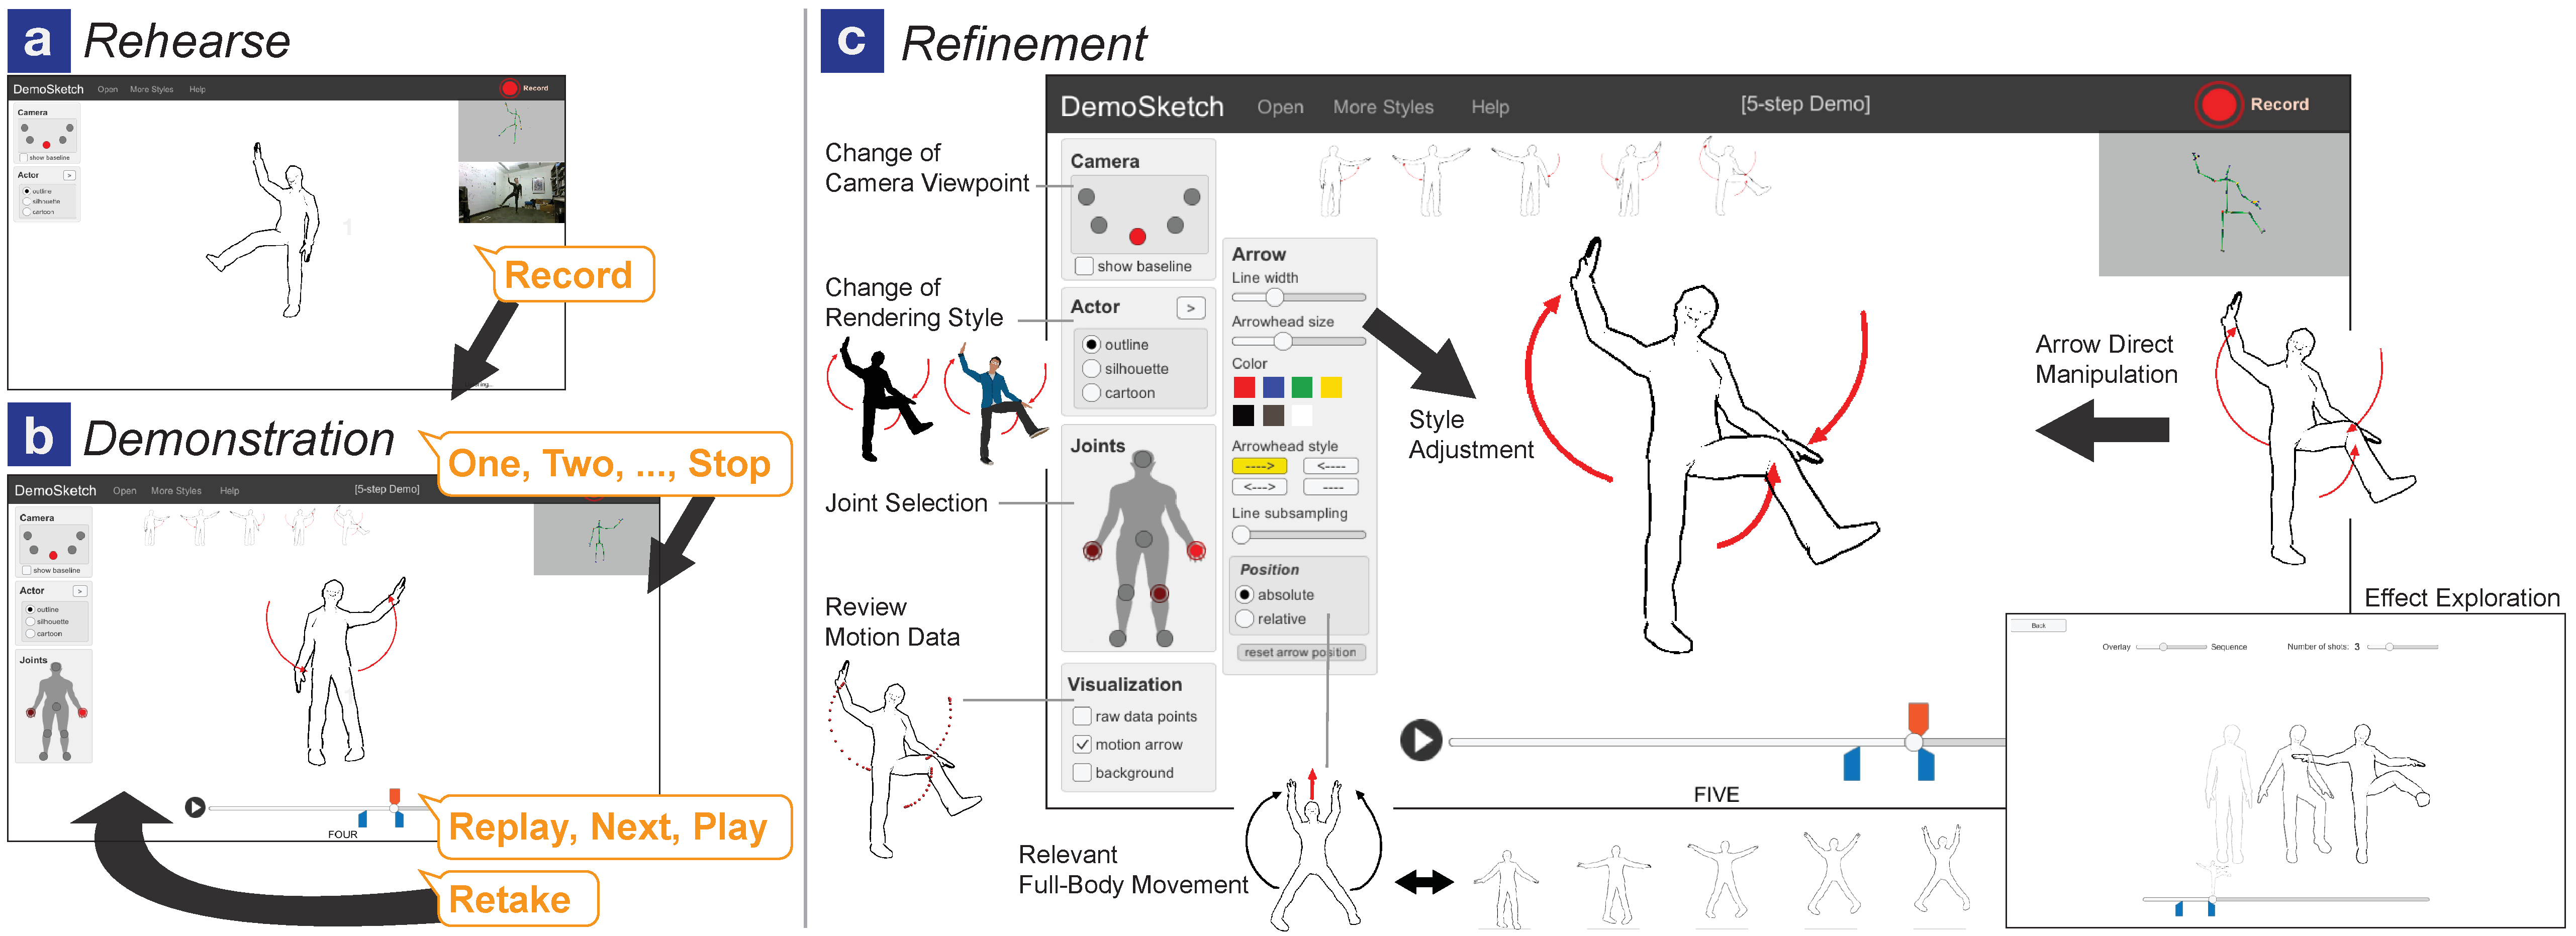
\includegraphics[width=\textwidth]{\demodraw/fig/ui/ui}
  \caption{\systemname{} authoring UI: Using the \phaseI{}, an author sees an avatar following her real-time movement (a). During recording (initiated by voice command ``Start''), real-time feedback shows the speech labels (b). Once a recording is completed by voice command ``Stop'', the motion visualization and a timeline are immediately available (c) for the author to review, and a step-by-step overview will be generated.}
  \dan{I changed figure start command to Start to match the video.}
  \label{fig:DemoDrawUI}
\end{figure*}

\section{Multi-Modal Authoring}
% \dan{Somewhere in this section need to justify need for motion re-taking and/or motion editing based on \textbf{three kinds of possible errors}: 1) user not happy with their own motion performance; 2) user not happy with quality of Kinect capture; 3) user not happy with system's motion segmentation or identified salience.}\bjoern{I'd add 4) based on illustration review, users decides to change performance to increase legibility.}

\systemname{} is designed for non-experts who cannot effectively or efficiently create concise motion illustrations motions using existing tools.
% This is achieved using two modes, the \phaseI{} and the \phaseII{}.
% \dan{The term ``phase'' implies a non-iterative sequential ordering. ``interface'' may not be good either if the UI is actually the same (I thought it was a bit different when they stood back for demonstration, but I guess not). Perhaps ``mode'' is best.)}
% \peggy{I agree and have changed the term in the paper}
To provide an overview of how the system works, we present a scenario in which a motion illustration author, Marie, creates instructions for an 8-step dance tutorial.

In her living room, Marie begins using \systemname{} with the \phaseI{} shown on her television by standing in front of a Kinect. In the center of the display, an avatar follows her movements in real-time (Figure~\ref{fig:DemoDrawUI}a).
 % with a smaller skeleton view and RGB video stream for recognition verification (Figure~\ref{fig:DemoDrawUI}-1b). \bjoern{I think you can get rid of the skeleton and perhaps also RGB video - those are debugging views for you.}
% \dan{just put one label for skeleton and RGB since these aren't a big focus}
This avatar is shown as an ``outline'' figure, but she could always change to different rendering effects like ``silhouette'' or ``cartoon,'' or select a different 3D human model later using our \phaseII{} (Figure~\ref{fig:DemoDrawRefinementUI}a).
% \dan{how does she select these while standing in front of the kinect? If she needs to use the \phaseII{} then let's talk about them there or have her pick them using the \phaseII{} before starting the demonstration.} \bjoern{yeah, i was wondering about this too}


\subsubTitleBold{Recording}
Marie starts recording her physical demonstration with the voice command \iquote{Start.} After a 3-second countdown, \systemname{} captures the position, orientation, and depth distance of her body (using Kinect's simplified 25 body joint model).
%
While demonstrating dance moves, Marie verbally indicates the count of each step with \iquote{one, two, three, and four,} just like she does when teaching a dance. The specific utterance is not constrained, Marie could use words like \iquote{right, left, shake, and clap.} A speech recognition engine captures these labels with timestamps and displays them in the interface (Figure~\ref{fig:DemoDrawUI}b).
Marie finishes recording by saying \iquote{Stop}.

\subsubTitleBold{Reviewing and Re-Recording}
After recording, \systemname{} automatically segments the motion around the speech labels and identifies salient joints. An illustration of the first step of Marie's demonstration is rendered with motion arrows, showing the path of the most salient joints. Figure~\ref{fig:DemoDrawUI}c presents an example illustration that shows how her right hand waves from bottom to the top, and the left on the opposite direction. She also notices three panels emerged: A timeline below shows the start, end, and key frame points used to generate the current illustration, a side panel shows the visualized joints; an step-by-step overview of step snapshots is created and added to a motion sequence list.
%
Marie can navigate to other illustrated steps by either saying \iquote{Next} or \iquote{Back}, or repeating one of the words she said during recording (like \iquote{three}) to skip to that corresponding step. To play an animation showing her continuous motion, she can say \iquote{Play} to play the current step only, or \iquote{Replay} to play the entire motion recording with each step visualization highlighted.

Once Marie reviews the steps, she realizes she should have exaggerated the hand motion in step 4. By saying \iquote{Retake Four,} Marie can re-record a partial sequence of movements including that step (e.g., redoing and saying ``Four'' and ``Five'').
When she ends the re-recording with \iquote{Stop}, the old illustration for that step is replaced with a new one (step four in this example) generated using the new motion recording.
%
% Furthermore, \systemname{} supports hand gestures for certain operations. For each step, \todo{Marie could adjust the start and end time of the motion using her left and right hands respectively.} By saying \iquote{Adjust}, she slowly moves her right hand to the right to extend the end time. She says \iquote{Done} to save the changes. She could always say \iquote{Cancel} to clear any recording or editing operation.
% No undo/redo
%
% TODO!! \dan{It would be so cool to have functionality to add and remove joints using the Kinect only: Marie finds that only her right hand was recognized as salient, but she wants a very subtle movement with her left hand to be shown too. She says \iquote{Add} while moving her left hand and the system adds her left hand's motion to the illustration. She can also say \iquote{Remove} to remove a joint from motion depiction.}

\begin{figure*}[t!]
  \centering
  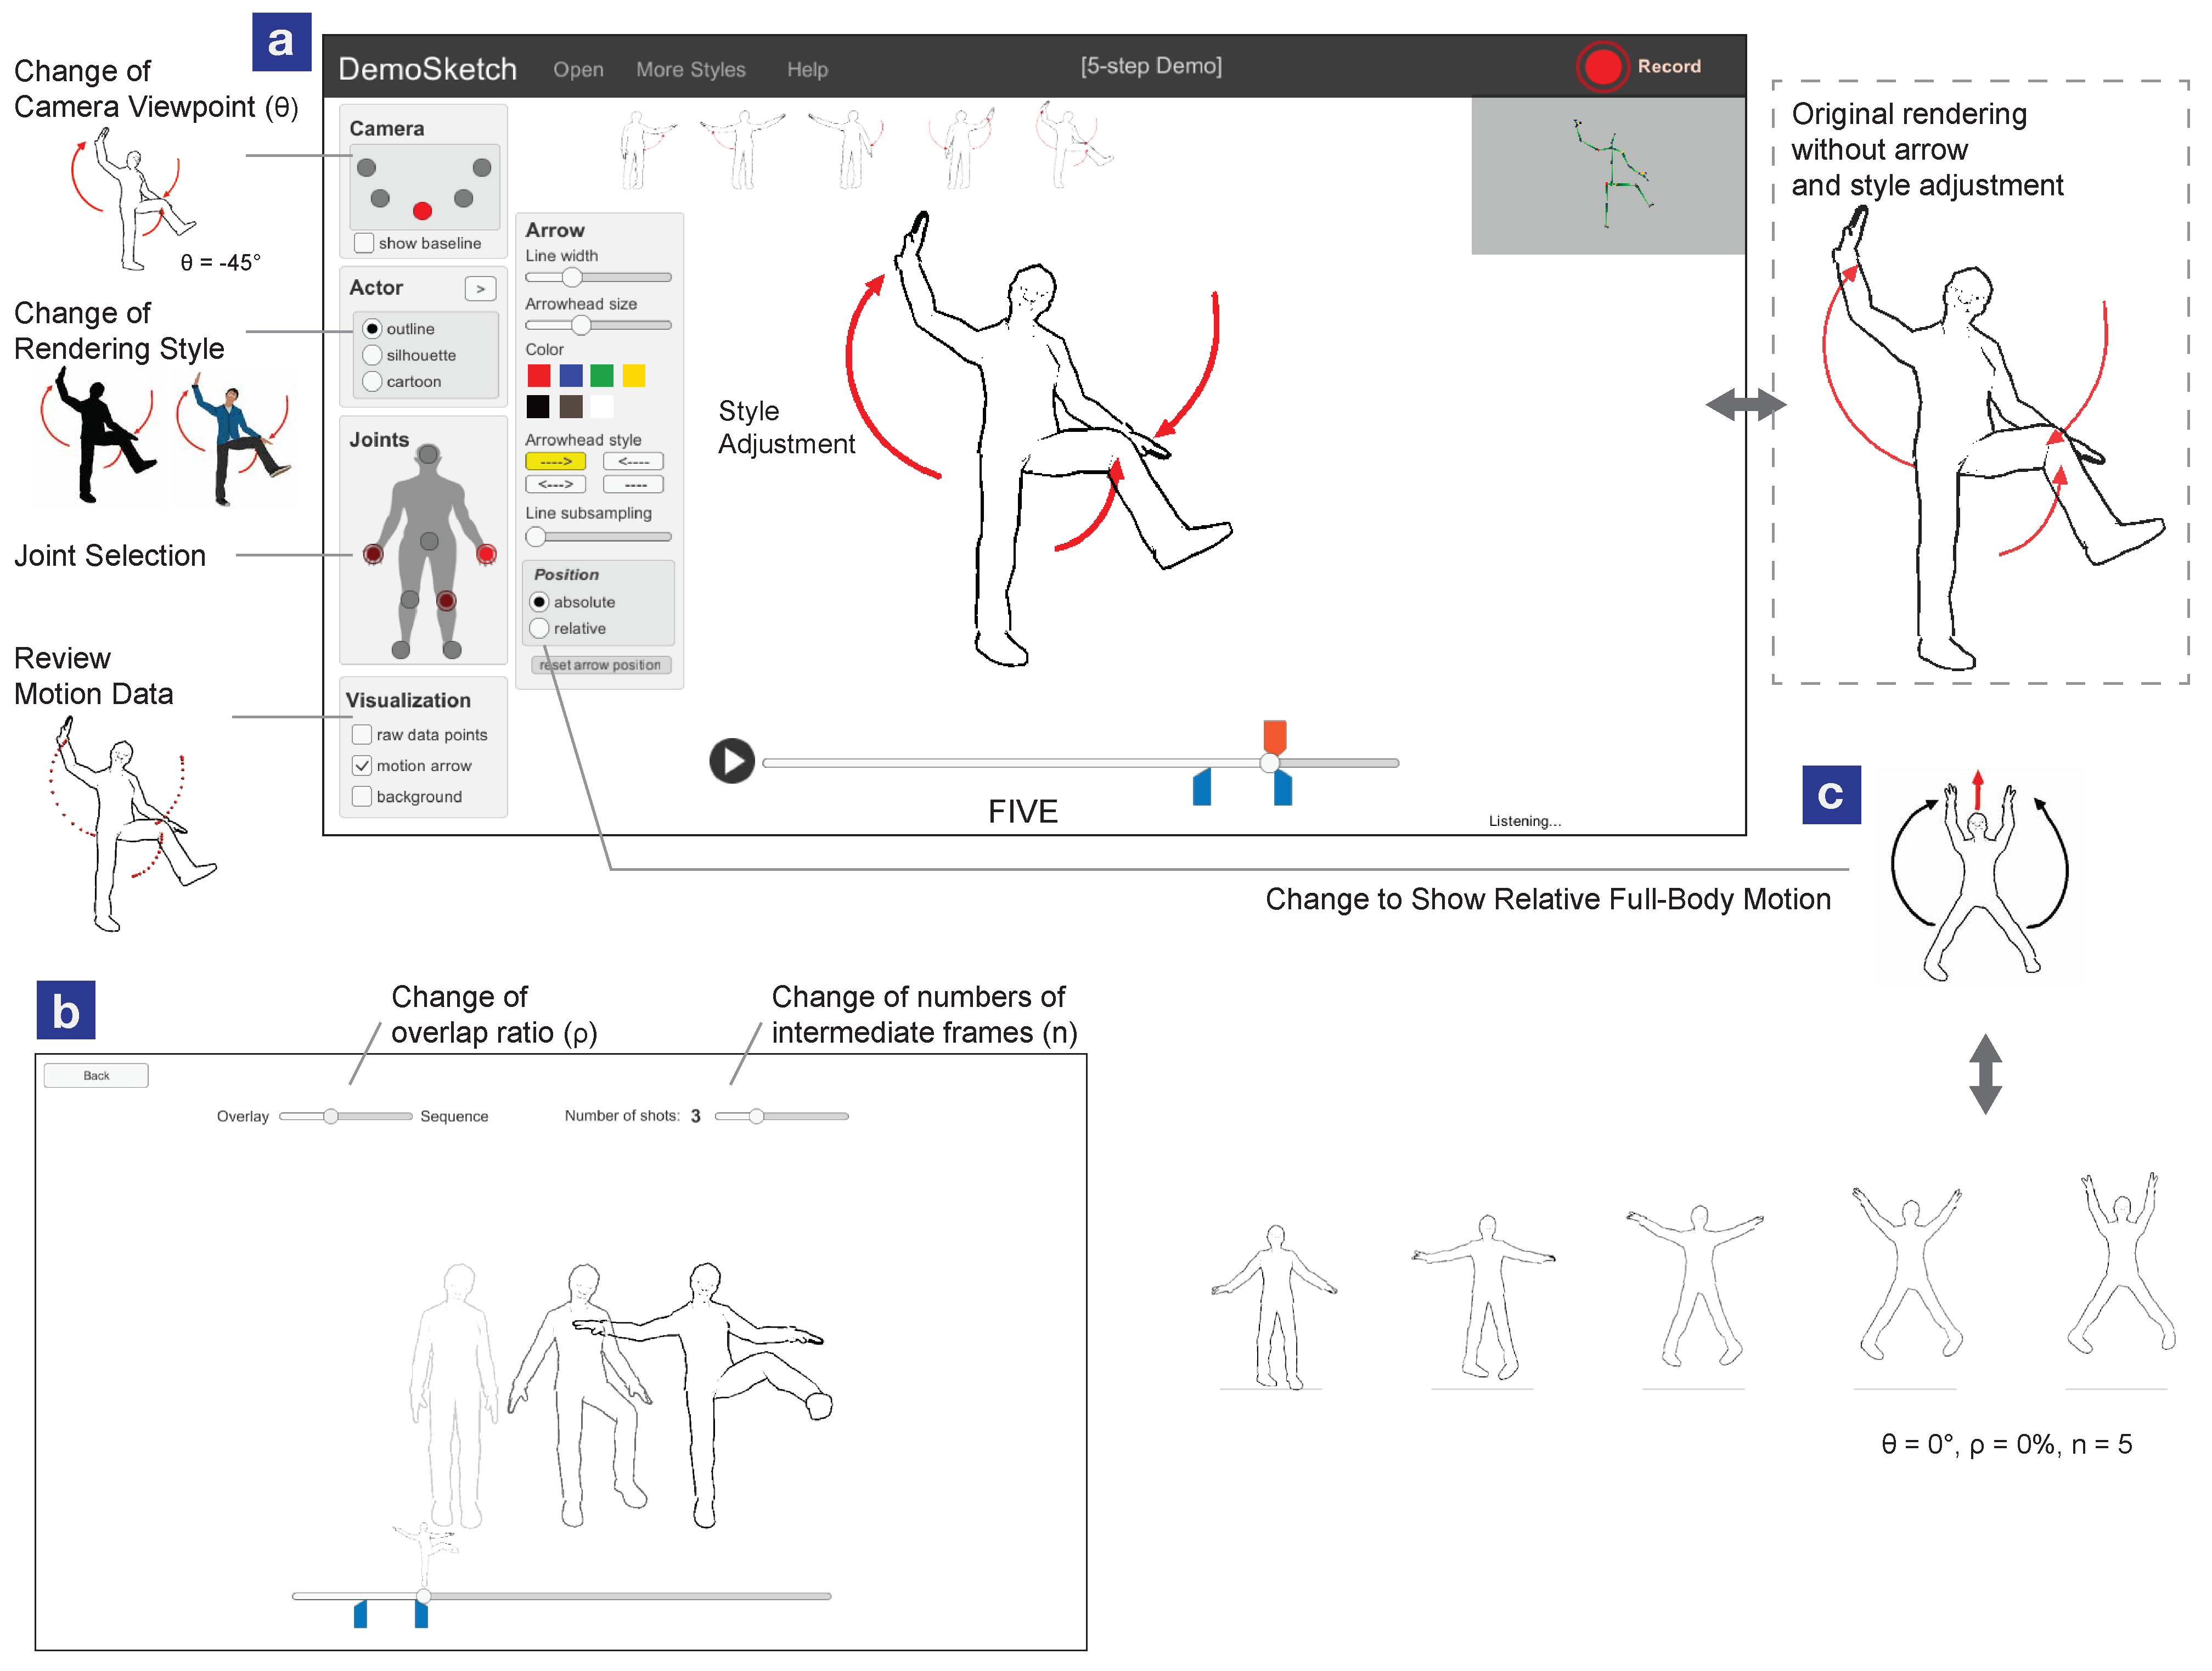
\includegraphics[width=\textwidth]{\demodraw/fig/ui/refinement_ui}
  \caption{Using \systemname{}'s \phaseII{}, the author can refine the visuals (a) and explore more illustration effects (b, c).}
  \label{fig:DemoDrawRefinementUI}
\end{figure*}

\subsubTitleBold{Motion Depiction Adjustments}
Once Marie is satisfied with her demonstration, she walks out of the capture area to her desktop computer. The system automatically switches to the \phaseII{} by revealing post-processing panels in a standard graphical user interface (Figure~\ref{fig:DemoDrawRefinementUI}a).
% \dan{so there are two interfaces!}
Using this interface, Marie can adjust several design parameters:
% \dan{I rewrite these to match parameters in figure 2 and added some as well.}
the arrow appearance can be refined, including line width, arrowhead size, and color;
the arrow offset can be adjusted with direct manipulation dragging; %to avoid overlap with the avatar figure
the camera viewpoint can be adjusted by orbiting the camera to a side or three-quarter view;
the joints used for motion paths can be added or removed using a panel;
% \dan{I put viewpoint in the ``context task'' in prev section, so may need to say something about not all context parameters needs to be adjusted in \phaseII{}. }
and the smoothed motion trajectory can be toggled on and off.
%
She could also select a different key pose and adjust the start and end times of a motion segment by dragging the markers on the timeline.
% \dan{if no relative vs. absolute adjustments, we may want to remove ``reference frame'' from figure 2}
% \peggy{Add something about relative motion here.}
%
In addition, Marie could explore other illustration styles like stroboscopic rendering by selecting numbers of intermediate frames and how they render in one diagram (Figure~\ref{fig:DemoDrawRefinementUI}b).
%
These results can be exported to image files containing the final motion illustrations. %replace vector files - possible but not implemented

% \dan{are there other motion styles? I commented out text that suggested that but I didn't think there were more than these two.}
 % for one or more steps to illustrate the continuous movement in one figure. By choosing ``More Styles'' from the menu, a dialog reveals for her to explore the effects.

% Beyond rendering motion arrows, the user decides the visualize a list of poses to compare with. She selects the option``Sequence'' from the menu and generates a stop motion sequence, with a default of 3 frames (Figure~\ref{fig:DemoDrawUI}A). She adjusts the start and end points of the whole motion via the timeline markers, and changes the number of shots and their distance to overlay the figures together (Figure~\ref{fig:DemoDrawUI}B).

% \dan{I would leave these out because they aren't really about post-processing design parameters:
% She could also reveal the raw, smoothened motion paths to confirm the captured data (Figure~\ref{fig:DemoDrawUI}B).
% To make sure the motion arrow renders the actual motion, she toggles the option ``motion path'' to reveal the original trails;}

% \fixme{\subsubTitleBold{Output}
% Finally, Marie chooses to output the generated illustrations of 8 dance moves to one step-by-step diagram. \systemname{} also provides other output formats, including step-by-step animated clips with the 3D model (where the viewing angles can be adjusted), or video snippets from the Kinect camera view (which only provides the front viewpoint).}
% \dan{not sure we should even talk about output formats other than motion illustrations since they're the only focus of this paper. We can talk about other formats like video and even MixT in future work or discussion. If you agree, then this whole ``output section'' can be reduced to a final sentence of the previous paragraph.  }

%!TEX root = thesis.tex
% Pipeline of the DemoDraw system: technical details

\begin{figure}[t]
  \centering
  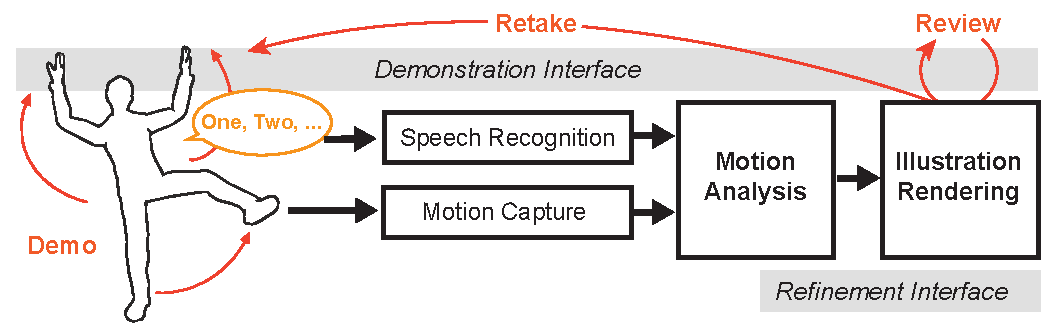
\includegraphics[width=0.8\columnwidth]{\demodraw/fig/pipeline/pipeline}
  \caption{\systemname{} System Components and Pipeline}
  % \dan{now that I understand the components better, we should emphasize motion capture component less since didn't make much contribution there.  I tweaked the figure to do this, and also highlighted the ``interaction pipeline'' (demo, review, retake) a bit better too.   }
  \label{fig:pipeline}
\end{figure}

\section{Generation Pipeline}

% \dan{I think we should downplay ``pipeline'' and emphasize ``system components'' ... pipeline sound very linear and non-iterative.}

%To support the described user scenario, we introduce our pipeline and system components shown in .
\systemname{} has four main components (Figure~\ref{fig:pipeline}):
%
a \emph{motion capture} engine to record joint data from the author's demonstration and apply it to a 3D avatar;
%
a \emph{speech recognition} engine to process speech input for commands and motion labels;
%
a \emph{motion analysis} algorithm to partition recorded motion and identify salient joint movements for each illustration segment;
%
and an \emph{illustration rendering} engine to visualize the avatar and motion segments with different effects.
% , and a module to handle user interaction.
%
% Our novel techniques enables motion segmentation by combining speech and motion inputs. Our interaction model allows users to modify the rendered illustrations interactively by demonstrations.
These components combine into an interactive and iterative system pipeline to translate demonstrations into motion diagrams.
A notable technical contribution is our motion segmentation algorithm combining speech labels and joint motion streams.
% \dan{I tweaked the two points above, old text is commented out in the tex}

% \dan{say something like our technical contribution is in motion segmentation (and maybe illustration rendering) }
%
\systemname{} is implemented using C\# in Unity 5. %\footnote{\url{https://unity3d.com}}.
It runs interactively on a Macbook Pro with Windows Bootcamp (2.5 GHz Intel Core i7 processor and 16 GB memory).
%
Below we describe the design and implementation of each component.

% ---------------------------------------------------------------

\subsection{Motion Capture}
% \dan{Call it ``Motion Capture'' component, with three sub components: Kinect, Avateering, and NPR}
% \bjoern{I moved NPR from capture to illustration rendering since it's a rendering technique.}
% \dan{good idea}

In support of our design goal to enable low-effort iteration within tasks, the motion capture component provides real-time feedback during demonstrations so authors can monitor their performance accordingly.
%\fixme{The raw joint data and RGB video stream are saved as csv and mp4 files for retrieval.}
%\dan{I put this here, but not sure we really need to state it at all. We don't really use the RBD video for anything either.}
% A central goal of our system is to enable average users to create illustration by physical demonstrations. As users might not necessarily have expertise to design illustration outcomes prior to a performance, it is important to provide real-time feedback for authors to observe the continuous motion captured effect and perform accordingly.
%
%\subsubTitleBold{Real-time Joint Data}
We capture position and joint angles of a simplified 25-joint skeleton using a Kinect2 sensor and the Kinect SDK 2.0. %\footnote{\url{https://dev.windows.com/en-us/kinect}}.
%Skeletal data of human body's 25 joints is captured in 3D, including head, shoulders, hands, and foot.
% At any given frame of motion capturing, our system gathers information about position, depth, and orientation values in meters for each of the 25 joints.
%Therefore, \systemname{} presents a 3D human model mirroring an author's movements in real-time while she stands in front of a Kinect sensor in a static, indoor scene (Figure~\ref{fig:pipeline}a).
%\dan{I commented a lot out here it didn't seem to add much beyond ``we capture using a Kinect'' (and just saying something like that is ok). }
%
%\subsubTitleBold{Motion Re-targeting}
The real-time joint data is applied to a generic 3D human model (an ``avatar'') using forward kinematics enabled by a modified Unity asset\footnote{\url{https://www.assetstore.unity3d.com/en/\#!/content/18708}}.
% \dan{I commented out a vague description of forward kinematics, I don't think we need it.}
% \bjoern{So the use of ``retargeting'' kinda raises a whole bunch of issues since motion retargeting is a big topic in animation. If bone lengths don't match between the actor's skeleton and the virtual model, contacts like clap or hand-on-head won't work. At a minimum state that we do not yet perform any smart retargeting to deal with changing segment lengths. I think the canonical reference is Gleicher~\cite{gleicher1998retargetting}.}
% \dan{yes, let's avoid saying ``retargeting''}

% When the motion data gets updated from the Kinect sensor, \systemname{} applies the joint information to a structured 3D human model (i.e., an ``avatar'') using forward kinematics in real-time. Given the human skeleton hierarchy from the body root (i.e., base spine) to the end of body parts (such as hand tips and feet), we compute the bone rotation angle to locate each joint to the target location in space. In this way, user can observe the avatar that follows her motion, which can also be viewed from any angle in a 3D space. This can be useful when user performs movements perpendicular to the Kinect camera \peggy{need a better way to frame this}.


% Based on our survey on existing practices of illustration design principles, it is important to make a character's appearance concise and clean. Often, outlining a human figure or showing in silhouette effectively preserves only essential information. Therefore, we apply Non-Photorealistic Rendering (NPR) techniques \cite{gooch1998non} to the 3D avatar in our engine that can be rendered and modified in real-time, including outline, silhouette, and flat-shaded colour (see Figure~\ref{fig:DemoDrawUI}-1d for examples).
% quaternion

% \subsubTitleBold{Implementation}
% This engine is implemented using Unity 5\footnote{\url{https://unity3d.com}} and the Kinect SDK 2.0 package\footnote{\url{https://dev.windows.com/en-us/kinect}} in C\#. Raw joint data and video stream from color frames are saved as csv and mp4 files for retrieval. Motion retargeting is achieved by a modification of a Unity asset\footnote{\url{https://www.assetstore.unity3d.com/en/\#!/content/18708}}. NPR shaders are applied to the 3D model for different rendering results.

% ---------------------------------------------------------------

\subsection{Speech Recognition}
Speech is used when recording a demonstration to label motions (e.g., ``one, two, ...'') and for recording and navigation commands (e.g. ``Start, Stop, Retake'' or ``Replay, Next, Play'') -- see Figure~\ref{fig:DemoDrawUI} for the speech commands that \systemname{} supports.
\dan{I made these consistent with new Figure 4}
%
We recognize both types of speech using the Microsoft speech recognition library\footnote{\url{https://msdn.microsoft.com/en-us/library/hh361572}} to process audio captured by the Kinect microphone array.
During recording, the start time, duration, and confidence of each motion label are logged for use in the motion analysis algorithm.
% https://msdn.microsoft.com/en-us/library/system.speech.recognition.recognizedaudio.starttime(v=vs.110).aspx
% \dan{how do you calculate delay? I thought this was a fixed constant determined by manual inspection.}
% \peggy{The api provides, but I didn't get to use it...}

%In addition, \fixme{a set of X voice commands} are recognized for non-sequential navigation .

%  addition to capturing and rendering user's continuous movements, \systemname{} considers instructor's existing practices of specifying motions using speech during a physical demonstration.
% By listening to the Kinect sensor's microphone array, \systemname{} integrates a speech recognition engine\footnote{\url{https://msdn.microsoft.com/en-us/library/hh361572}} to recognize user's speech input in real-time. Information of a detected spoken word, including the timestamp, delay, and confidence, is captured to be used for motion analysis and to support \systemname{}'s multi-modal interaction.
%
% Can implement: go more than one word and combine (e.g., turn to the right)

% ---------------------------------------------------------------

\begin{figure}[!t]
  \centering
  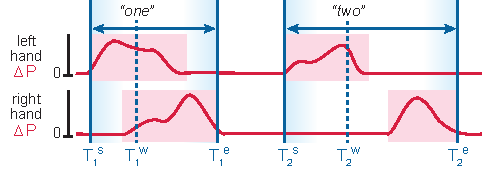
\includegraphics[width=0.8\columnwidth]{\demodraw/fig/motion_analysis/analysis2}
  \caption{Illustration of motion analysis algorithm (two joints shown due to space): significant moving periods of joint movements (pink) are mapped to speech labels to define motion segments (blue). Note the right hand period is mapped to \iquote{two} because it begins shortly after the left hand period.}
   \label{fig:segmentation}
\end{figure}

\subsection {Motion Analysis}
% \dan{Would be good to get a component name to include joint salience identification too.  ``Motion Segmentation and Joint Salience Identification'' component is too long, how about something more simple and general like ``Motion Analysis'' with subcomponents motion segmentation and joint salience.}

Our motion analysis algorithm translates a multi-part demonstration recording into a sequence of labeled time segments, each with one or more salient joint motions and a keyframe of joint positions for a representative body pose (see Figure~\ref{fig:segmentation} for an illustration of the approach).
Formally, given a set of $n$ speech labels $\{w_1, w_2, ..., w_n\}$ where each ends at latency-corrected time $\{T_1^w, T_2^w, ..., T_n^w\}$, our algorithm associates each speech label $w_i$ with a \emph{motion segment}, of which the start and end time are denoted as [$T_i^s$, $T_i^e$] where $T_i^s \leq T_i^w \leq T_i^e$. Each motion segment includes a set of $k$ salient joints $\{j_i^1, ..., j_i^k\}$ and keyframe time $T_i^{key}$ between [$T_i^s$, $T_i^e$].
It is then sent to the Illustration Rendering engine to create a motion illustration in a multi-part sequence.

Human motion segmentation and activity understanding has been well studied in computer vision and graphics \cite{Aggarwal:2011:HAA:1922649.1922653}. We adopted a spacetime approach to identify salient motion sequences in 3D space.
%
However, in our scenario such as dancing, movements may not necessarily encode a semantic meaning for automatic recognition, such as ``walking'' or ``throwing (a ball)'' in previous research. Therefore, our approach combines the user's speech labels, similar to a scene segmentation method used in DemoCut~\cite{Chi:2013:DGC:2501988.2502052}.
%
We make two assumptions about the synchronized data streams of speech labels and joint movements:
1) authors make short pauses between motions to be grouped, i.e., $T_i^e < T_{i+1}^s$, and
2) the speech label utterances overlap or closely occur with at least one joint motion;
% step-by-step movements are clearly segmented without an overlap.
%
These assumptions are practical since authors often pause for a moment to prepare for demonstrating the next movement in a step-by-step sequence.
% , or reposition their body without those movements being assigned to any label.

% where $T_s \leq T_w \leq T_e$,

% For a motion label detected by the speech recognition engine at time \(T_w\) (e.g., step ``One'' or a gesture ``Swipe''), \systemname{} automatically identifies an appropriate motion segment for visualization as follows: It analyzes the motion data in order to identify the start and end time of this segment [\(T_s\), \(T_e\)] where \(T_s \leq T_w \leq T_e\), a set of salient joints \({J_0, ..., J_n}\), and a representative pose at \(T_k\) associated with this speech label. Figure~\ref{fig:segmentation} shows one example of a right-hand movement segmented by the following approach: \bjoern{What instant in time does \(T_w\) represent? The beginning of a word? The end? Some time after the end of the word once recognition has completed? Seems fairly important - otherwise I have no idea if \(T_s \leq T_w \leq T_e\) is a reasonable assumption.}

% EUCLIDEAN DISTANCE
\subsubTitleBold{Motion Segmentation}
To determine a motion segment of [$T_i^s$, $T_i^e$] for each speech label $w_i$ that ends at $T_i^w$, we begin by identifying all \emph{moving periods} of significant joint movements (pink rectangles in Figure~\ref{fig:segmentation}) for 8 joints $J$: the 5 end-effectors (head, hands, feet), 2 knees, and the body root.
%
To filter jittery movements, joints are considered moving if smoothed inter-frame differences in absolute Euclidean distance are greater than a threshold.
%
Specifically, for each joint $j \in J$ of a frame $r$ at time $t$, the average difference in position between two adjacent frames $\Delta P = |P^r-P^{r-1}|$ is computed over the subsequent half second (15 frames).
%
If this moving average is greater than 0.05$m/s$, then joint $j$ of a frame is labeled as ``moving'', marked as $m_j^r$.
This is repeated on all frames and all joints.
Next, of the entire motion recording for joint $j$, we combine all the consecutive $m_j^r, m_j^{r+1}, ...$ into a joint moving period $M_j$.
% \dan{any extra hacks to join or filter out very small periods of movement like just a few frames? If so, explain here.}

Once a list of moving periods $\{M_j^1, M_j^2, ...\}$ for joint $j$ is determined, we begin labeling each $M_j^m$ at [$T_{m}^s$, $T_{m}^e$] to map to a speech label $w_i$ at time $T_i^w$ where $T_m^s \leq T_i^w \leq T_m^e$. In other words, the speech utterance occurs during or near to a joint movement (illustrated as dashed lines crossing pink rectangles in Figure~\ref{fig:segmentation}).
%
% Salient joint marking covered in the next paragraph ...
%Mark \(J_i\) as salient.
%
% If a movement overlaps with two labels (i.e., a continuous movement without a pause in between beyond our general assumption),
%
% \dan{do you have any rules to prevent a period of joint movement to be mapped to multiple speech labels?}
%
% Any unmapped periods ending less than $\epsilon$ before a motion label time, where $\epsilon = $ 1s defined earlier, or beginning less than $\epsilon$ after a motion label time, are also mapped to that label.
% \dan{See if what I wrote above makes sense, I was trying to interpret ``or 2) if an earlier segment that ends within a pause threshold is not mapped. A second pass of analysis after recording will examine if a segment shown after the label should be mapped to this label.'' }
%
% \fixme{After all the moving sequences of a joint is identified, \systemname{} concatenates these elements and finds the earliest frames at \(T_s\) and latest frame at \(T_e\) as the start and end times of this motion segment. Mark this as a salient joint \(J_i\).} \bjoern{revisit - i find this unclear, but I'm also tired.}\dan{I can't figure it out either, but I think it needs to be explained here}
%
After all moving periods are mapped to speech labels for all major joints, the start and end time [$T_i^s$, $T_i^e$] of the motion segment for label $w_i$ are set to the minimum start time and maximum end time across all mapped joint movement periods.
%as [$\min_{\forall j \in J} T_jm^s$, $\max_{\forall j \in J} T_jm^e$].
% \dan{the sentence above is my guess at what this means (same as what Bjoern guessed)
% ``Our algorithm repeats this segmentation for all the major joints. If there are multiple salient joints, combine and adjust [\(T'_s\), \(T'_e\)] for this motion segment.'' \bjoern{How do you do the adjustment? do different joints have individual start and end times, or do you take the min of all start times and the max of all end times?}}

\subsubTitleBold{Joint Salience Identification}
The salient joints $\{j_i^1, ..., j_i^k\}$ are defined by the set of all joints that were mapped based on significant moving periods.
% \dan{any other rules or hacks to do this?}

% \systemname{} analyzes a motion recording for significant motion changes using spatial thresholding of key joints. To concisely visualize body motion, we selected a subset from the 25 joints by their relative distance of a human body. For example, shoulder center can be represented by the head movement, and therefore trace only the latter joint. \bjoern{This is vague - which joints did you select? Why is this ``concise''? I don't understand the sentence about shoulders and heads at all. Maybe show a figure and highlight which joints you check.}
%
% For each joint, we calculate the Euclidean distance of joint locations in adjacent frames: $\Delta P = |P_t-P_{t-1}|$. If the average distance of a consecutive sequence within a moving window (set as 2 seconds) is over a difference threshold, it labels this as a moving joint sequence. \bjoern{what do you mean by average distance? do you just add up all frame differences for 2 seconds and divide by \# of frames? What is the difference threshold you empirically determined? What are the times $[T_{start},T_{end}]$ you find? }

% MATCH WITH SPEECH + FIND IN/OUT POINTS
% Next, our algorithm maps a moving joint sequence to this speech label if: 1) the sequence in time overlaps with the label's time \(T_w\), i.e., the movement is continuing, or 2) if an earlier segment that ends within a pause threshold is not mapped. A second pass of analysis after recording will examine if a segment shown after the label should be mapped to this label.
% %
% After it identifies all the moving sequences of a joint, \systemname{} concatenates these elements and finds the earliest frames at \(T_s\) and latest frame at \(T_e\) as the start and end times of this motion segment. Mark this as a salient joint \(J_i\). \bjoern{revisit - i find this unclear, but I'm also tired.}

% MULTIPLE JOINTS
% \subsubTitleBold{Joint Salience Identification}
% Our algorithm repeats this segmentation for all the major joints. If there are multiple salient joints, combine and adjust [\(T'_s\), \(T'_e\)] for this motion segment. \bjoern{How do you do the adjustment? do different joints have individual start and end times, or do you take the min of all start times and the max of all end times?}

% KEY FRAME
\subsubTitleBold{Key Pose Selection}
A key pose is used to represent a motion segment in an illustration. Based on our informal experiment, it is often the end state of movements as motion arrows are pointed toward this end goal (see the Figure~\ref{fig:pipeline} for example). Therefore, we set a key pose at a time near the end of a motion segment, specifically $T_i^{key} = T_i^e - 0.5$ second.
% \dan{should mention keyframe position in formative study section}
% \peggy{confirmed, and in figure 2}
% Therefore, we selects a frame \bjoern{x frames} from the out point \peggy{no intelligence here... how do we better describe?}.

\subsubTitleBold{Motion Retake}
When retaking a partial demonstration with one or more speech labels $\{w_i', w_{i+1}', ...\}$, the full motion analysis algorithm is run on the new recording. New motion segments then replace the original segments by mapping $w_i'$ with $w_i$.

% ---------------------------------------------------------------

\subsection{Illustration Rendering}

The Illustration Rendering engine generates a motion illustration for each motion segment of speech label $w_i$ (bounded by [$T_i^s$, $T_i^e$]). There are two related rendering tasks: the body pose and the motion depiction style.

\subsubTitleBold{Body Pose}
The body pose is determined by all joint positions at keyframe time $T_i^{key}$.
We use standard Non-Photorealistic Rendering (NPR)~\cite{gooch1998non} techniques to render the 3D human model in a stylized manner that abstracts away distracting details. Specifically, we support contour-only, filled silhouette, and flat-shaded rendering styles
% Following the principle of clarity through simplicity, Non-Photorealistic Rendering  \cite{gooch1998non} algorithms are used to render the 3D human model as a contour, silhouette, or flat-shaded colour
(see Figure~\ref{fig:DemoDrawRefinementUI}a left for examples).
% \dan{any more details? Unity asset used? tuning parameters? Is it fast?}

\subsubTitleBold{Line and Arrow Depiction Style}
Based on Cutting's criteria~\cite{cutting_representing_2002} and our survey of motion illustrations, we use lines with arrowheads as the default depiction style for visualizing joint movements.
This style is rendered as follows:
%
For each salient joint of a motion segment, the absolute joint positions in world space over the period [$T_i^s$, $T_i^e$] are used to construct a 3D poly-line using Catmull-Rom interpolation.
% \dan{can smoothing still be turned off?}
% \peggy{current not}
Two 3D cones are positioned collinear with the last two polyline positions to form arrowheads for both the beginning and the end of a line.
%
Although the poly-line is 3D, it is shaded to appear 2D.
%
All arrows are colored red by default to contrast with the avatar, a common technique for layering information~\cite{tufte1990envisioning}.
% \dan{and rendered to be always ``in front'' of the body.}
% \peggy{currently does not consider camera viewpoint, so no}

For some motions, visualizing absolute joint positions might not be suitable.
For example, for a two-foot jump with a two-hand waving motion (see Figure~\ref{fig:DemoDrawRefinementUI}c), our algorithm will mark all major joints as salient and generate multiple arrows showing the jump movement, but fail to convey the hand waving.
%
Authors can choose to visualize joint motions \textit{relative} to the spine instead,
triggering the same motion analysis algorithm described above to be re-run using relative motion.
In this way, the same movements would be shown more concisely with a single up arrow (for the overall jump direction) and two curve arrows (for the hand movements).
%The joint data will be re-computed based on the offset distance to the spine position. The result illustration, in this case, can be more concise by showing only the spine motion.

\subsubTitleBold{Other Adjustments}
Authors can review the results using the \phaseI{} or \phaseII{}. With the latter, line weight, arrowhead sizes, and color can be adjusted and re-rendered in real-time using graphical widgets (see Figure~\ref{fig:DemoDrawRefinementUI}a). Arrows can also be re-positioned to increase the offset ($\delta$) by direct manipulation dragging.
%
Considering some movements cannot be easily seen from the default front camera viewpoint (such as those parallel to the XZ plane, see Figure~\ref{fig:teaser}c top-right), our UI enables the selection of four other camera angles ($\theta$), including three-quarter front views (45$^{\circ}$ and -45$^{\circ}$) and profile views (90$^{\circ}$ and -90$^{\circ}$), all at the eye level. These discrete choices simplify control, but of course it would be possible to select any viewing angle given the 3D avatar and joint information. By default, 8 main joints are analyzed and illustrated, but any of the 25 body joints can be explicitly selected for illustration using the interface.

\subsubTitleBold{Stroboscopic Depiction Style}
Cutting~\cite{cutting_representing_2002} noted stroboscopic effects are also effective, and we found examples of illustrations with a sequence of overlaid semi-transparent body poses in our survey.
%
Therefore, authors can select a stroboscopic depiction style in the \phaseII{} (see Figure~\ref{fig:DemoDrawRefinementUI}b).
The style is rendered by compositing multiple semi-transparent renderings of intermediate body poses between $T_i^s$ to $T_i^e$ behind a rendering of the representative pose at keyframe time $T_i^{key}$.
Authors can adjust the number of intermediate poses $n$ (the default is 3 poses) and the horizontal overlap ratio $\rho$ between intermediate pose renderings can be adjusted to stack them up ($\rho=100\%$) or spread them out ($\rho=0$ is the default).

% Authors can then selectively combine these frames by specifying visual parameters, including numbers of frames to show, distance between frames, and whether to apply motion arrows. Our system will automatically adjust the distance and transparency values of selected frames and compose into a diagram.

\subsection{Results}
The \systemname{} pipeline is capable of generating expressive and clear motion illustrations. In Figure~\ref{fig:teaser}c, motion arrows show the upper body motion (top left), hand waving back and forth (top middle), and hand circular motion (bottom right). Whole body motions can also be visualized (bottom left), and can be especially helpful when motions are best viewed from a different angle, such as the side view (top right).
%
In Figure~\ref{fig:teaser}d, stroboscopic effect depicts the transition from the start pose to the end pose, which can be rendered as a sequence (top left) or in one combined pose (bottom left). A combination of this effect with motion arrows creates a compact, integrated illustration (top and bottom right).

% \dan{Talk about how expressive this pipeline is referring to diagrams shown in figure 1, the appendix, etc.}

\dan{Disclose what happens if assumptions don't hold or other problems with the pipeline. (this paragraph may migrate elsewhere).}

% ---------------------------------------------------------------

% -- Rebuttal --
% * Camera positions can present motion parallel to the XZ plane (R1), see Fig 1c top-right.
% * We do not embed color coding (R1,R2); we integrate "CMC l:c color differencing" to automatically avoid arrow colors visually similar to avatar colors.
% * 8 major joints are selected to give users higher-level control, but the system tracks all 25 detailed joints that can be revealed via the Refinement UI (R2).
% * Arrow path points are not sampled before Catmull–Rom interpolation (R1). It's simple, but it works because motions are often taken in 0.5s to 1s. We agree that sharp direction changes could be smoothed over: we can discuss alternate sampling methods like finding points with local min/max derivatives.

%!TEX root = ../thesis.tex
\section{Evaluation}
To evaluate the DemoWiz design, we conducted a controlled experiment in which participants recorded and edited a demo video, and gave a presentation with the edited video. Specifically, we wanted to see if presenters would evaluate their own performances higher with the support of our augmented visualizations and control of timing.

\subsection{User Study}

\subsubsection{Baseline Condition: DemoWiz without Visualization}
Since DemoWiz allows for rapid editing of the video, it would have been unfair to compare it with a conventional video player without supporting any editing during the rehearsal phase. We therefore modified our system to serve as the baseline condition, providing participants with the same lightweight editing of the video in each condition. However, during presentation, the baseline condition was similar to a conventional video player that shows only the video without event timeline and augmented visualizations. It also did not support the \textit{stop} markers and \textit{text notes}, i.e., participants could only adjust playback speed of each segment and add variable length \textit{pauses}. During presentation, participants only saw the video with a traditional timeline. They could, however, pause (or stop) and resume the video manually at any time during playback.

\subsubsection{Study Design}
We conducted the study as a within-subjects design in a usability room. After recording and editing a video using the same system, each presenter gave a presentation with both systems to an experimenter. To control the effect of order and learning, we prepared two tasks that included similar interaction flows and counterbalanced the order of the two systems—DemoWiz and Baseline—-but we fixed the order of tasks. Even though presenting to a single audience member in a usability room is not the same as using the system with a large conference audience, it is important to control the tasks and presentation as closely as possible to understand the relative benefits of the system in comparison with a baseline condition.

For each condition, we observed and coded the \textit{timing} of narration that matched the video content and noted the time in seconds when an event was described \textit{before}, \textit{at}, or \textit{after} the action happened in the demo video. We also marked obvious \textit{breaks} between narrations, \textit{errors} when the narration was not about the current or following events (e.g., discussing actions in a different order than they actually occurred), and \textit{misses} when an important action was not mentioned. To avoid unconscious bias that might influence the coding of the videos, we neutrally named the recordings and coded them all in a batch. We focused on objective timing measurements as much as possible, measuring deviation from specific video events and their corresponding narrations down to a second. Finally, we gathered qualitative feedback through satisfaction and preference questionnaires.

\subsubsection{Participants}
We recruited 12 participants (10 males and 2 females) from a software company. However, we excluded the data from two participants (1 male and 1 female); one was due to a software bug during one condition and another was because the participant requested to restart a presentation in one condition. The average age of the effective 10 participants was 37.3 ranging from 24 to 64 years of age. We recruited participants who had experience at showing a software demonstration to an audience such as giving a presentation at a conference. Four participants were native English speakers and the rest were fluent in English. The expertise of participants included audio processing, computer graphics, human-computer interactions, machine learning, networking, and software engineering. Each participant was compensated with lunch coupons worth \$20.

\subsubsection{Procedure and Tasks} Each session consisted of one training task and two experimental tasks. For the training task, to introduce the common features for recording and editing the video, we designed a simple workflow of five steps to demonstrate editing of a slide using PowerPoint. The experimenter briefly demonstrated an example and then introduced the recording program that captured the screen. Participants were then asked to practice and record using the recording program.

The two tasks consisted of a similar sequence and interactions: 1) searching with Bing Maps to show the 2D map view and the Bird's Eye view, looking for a restaurant, and navigating to the interior view of a specific restaurant; and 2) searching with Google Shopping to show the search results with the Grid view, filtering and voting for reviews, and navigating the 3D product view of an espresso machine. For each task, we provided a specific scenario along with a list of subtasks. The experimenter walked through this list with participants to ensure that they could easily find the features that needed to be demonstrated. Participants were then asked to practice (3-5 minutes), record (about 2 minutes), and rehearse and edit (5-10 minutes).

To help simulate a conference setting where participants would not be able to present immediately after having recorded a demonstration, we inserted an intentional 1-minute gap between rehearsal and presentation. During this gap before giving the presentation, we asked participants to watch a conference showcase video. Participants were then asked to stand up and gave a 2-3 minute presentation to the experimenter in a usability room.

After each task, participants filled out a questionnaire of 8-10 questions asking about their experience (8 for the Baseline condition, and 10 for the DemoWiz condition). At the end of the session, an online questionnaire was provided for them to present overall preferences and leave comments. Each session lasted about 1.5 hours.

\subsubsection{Experiment Setup}
Each participant used a desktop computer running Windows 7, Expression Encoder 4 for screen recording, and a web browser for the DemoWiz user interface. A regular mouse and keyboard were provided, along with two 27-inch displays, one for editing (during rehearsal) and showing the audience view (during presentation), and the other for the presenter view on a stand-up table. The resolution of both displays was 1920×1200 pixels. The average captured screen area was 1311×857 pixels. In the presenter view, the video resolution was within 1000×600 pixels; in the audience view, the screencast videos were resized to fill the entire display with at least 100-pixel wide border in black. During the study, the experimenter stayed in the room, providing instructions and sitting behind the participants during the recording and editing phases.

% ---------------------------------------------------------------

\subsection{Results}
Ten participants successfully recorded, rehearsed, and gave a demo with both systems.

\subsubsection{Subjective Preference}
Figure~\ref{fig:demowiz_likert} shows the average subject responses (on the 7-point Likert scale) from presenters for both systems. We analyzed these subjective responses using a Wilcoxon signed-rank test. We found significant differences in responses for ease of narration (DemoWiz µ = 6.2 over Baseline µ = 4.5, \textit{p} = .018) and ease of presentation (6.4 over 5.2, \textit{p} = .048). We also found marginally significant differences in participants' overall satisfaction with their presentations (5.5 over 4.7, \textit{p} = .062). Participants also tend to agree that DemoWiz helped them interpret timing (6.1 over 4.4, \textit{p} = .067).

In addition, 9 out of the 10 participants preferred DemoWiz to the system without visualization and would choose to present with DemoWiz if they were asked to give a public software demo; the remaining participant indicated no preference for both questions. The general feedback was also encouraging. For example, P1 commented \iquote{Awesome system. I'd use it today.} and P5 \iquote{felt more confident in being able to present what I wanted to.}

\begin{figure*}[t]
  \centering
  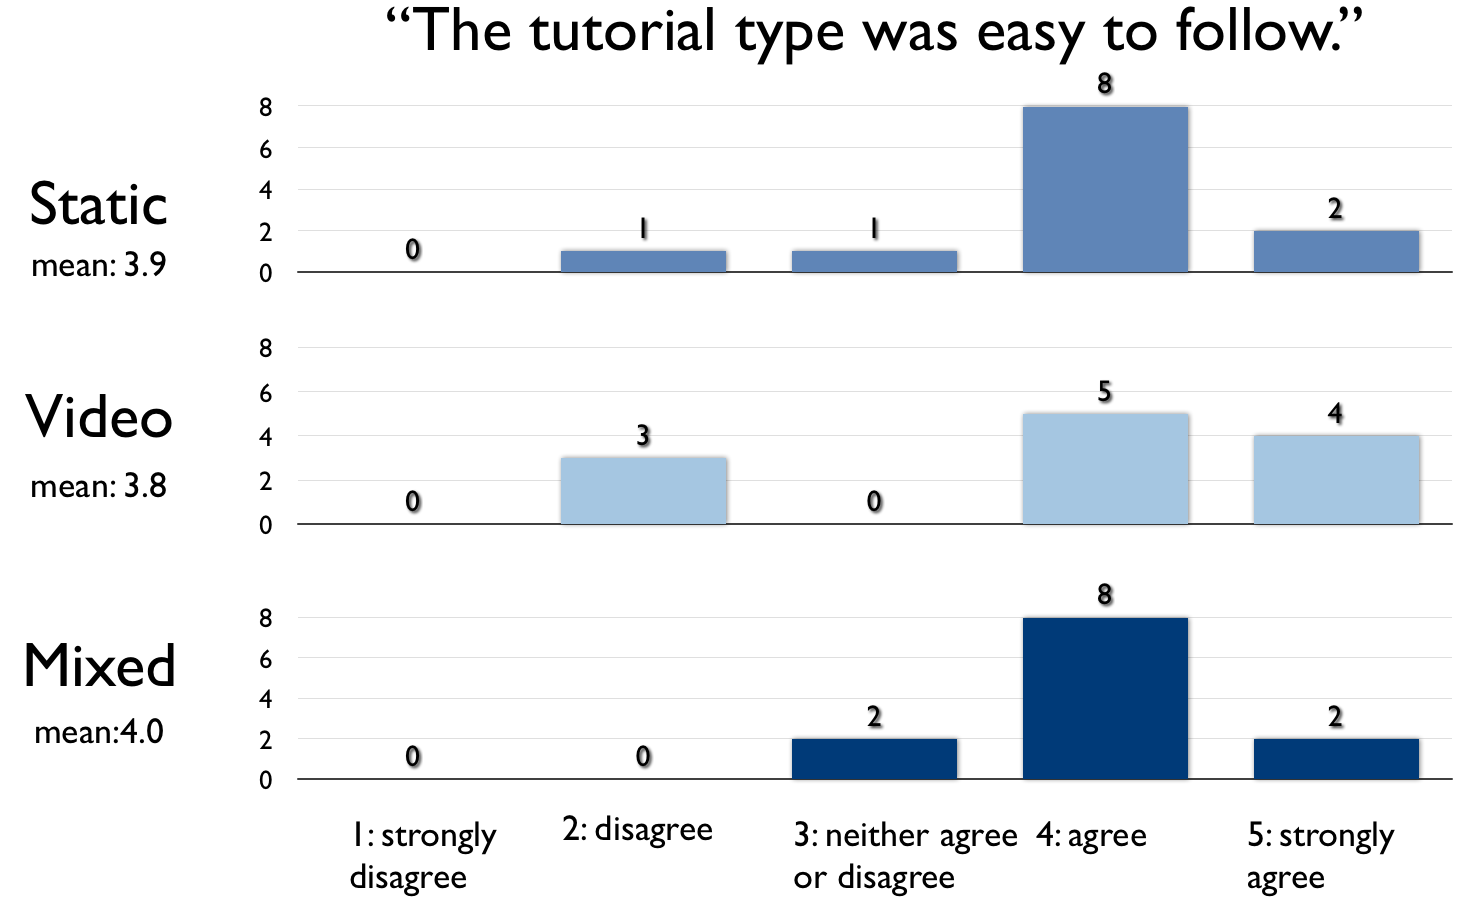
\includegraphics[width=\textwidth]{\demowiz/fig/results/likert}
  \caption{User feedback from questionnaire on the 7-point Likert scale.}
  \label{fig:demowiz_likert}
\end{figure*}

\subsubsection{Visualization as a Supportive Cue}
Participants answered that they were able to understand DemoWiz visualization of input events (µ = 6.0) and found it supportive for their presentations (µ = 6.3). They also commented that the DemoWiz visualization supported the presentation in various aspects: \iquote{the visualization reminds of the order of the content} (P1), \iquote{Really liked the ability to know what was coming up} (P2), \iquote{It provides better insight of the progress of the video} (P6), and \iquote{viz gave me an idea about timing or something I was going to forget to say} (P9).

\subsubsection{Narration Timing}
We coded the 20 recordings of participants' final presentations to observe the timing of narration of each action in correspondence with the video content (11 key events for both tasks). With DemoWiz, participants tended to \textit{anticipate} the upcoming events rather than talk afterwards, where the average timing was -0.1 seconds with DemoWiz (i.e., narrated the action before it happened) and 0.4 seconds with the Baseline condition (i.e., explained the action after it was shown). We found a significant difference in the number of times that events were anticipated by the narration, co-occurred, or occurred after the fact ($\chi $\textsuperscript{2}\textit{(2,220) = 8.6, p = .01}, see Figure~\ref{fig:demowiz_results_timing}).

In general, this supports our suspicion that DemoWiz would help in anticipating an event as opposed to talking about it after it occurred. More important though, was how often a narrator spoke about an event within several seconds of when the event actually occurred. By defining \textit{better} timing as when a presenter's explanation came within 2 seconds of a shown event (either prior, exact, or after), there was marginal significance by condition (\textit{p} = .089 with DemoWiz performing better). In addition, with the Baseline condition, the timing of narration was less consistent and off more, varying from 6 seconds early or 10 seconds late with a variance of 3.9 seconds, in comparison to the DemoWiz condition with at most 3 seconds early to 3 seconds late and a variance of 1.9 seconds.

Five participants had an obvious \textit{error} (forgot the next action or incorrectly narrated another action), had a long \textit{break} (waiting for more than 2 seconds until the action was made), or \textit{missed} an action (did not explain an important feature) when presenting with the Baseline condition. On the other hand, in the DemoWiz condition no errors were made, and there were only one long break and one miss from two different participants, respectively.

Participants' comments also support the fact that DemoWiz helped presenters anticipate the upcoming events. P7 explained, \iquote{(I) felt better able to time my speech to coincide with visual events, rather than trailing after them. Without the event visualizations, I felt like I was talking about what the audience had just seen, rather than having my words and visuals combine to a single message.}

\begin{figure*}[t]
  \centering
  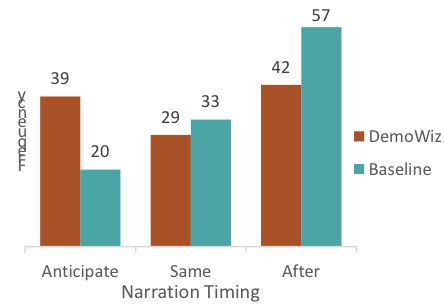
\includegraphics[width=\textwidth]{\demowiz/fig/results_timing}
  \caption{The number of times events were anticipated by the narration, co-occurred, or occurred after the fact.}
  \label{fig:demowiz_results_timing}
\end{figure*}

\subsubsection{Editing Experience}
We collected comments on the workflow. Participants found it easy to record (µ = 6.4) their demonstrations with DemoWiz. For editing features, they found it easy to edit in general (6.6), including controlling the playback speed (6.5) and adding pauses and stops (6.5), but it was less easy to add text notes (4.8); only two participants used this as reminders.

Although using different strategies, all of the participants adjusted the playback speed for matching their narration. Some sped up whenever possible and added stop markers for transitions; some slowed down the repetitive actions (such as drags) to demonstrate effects. P6 said, \iquote{I really liked being able to add ‘stop' events so I could \'fake\' my demo better.} DemoWiz made it easy for participants to separate the capturing and presentation preparation as P5 explained, \iquote{Overall, recording was very easy. In fact, as I got to the second task, I realized that I really don't need to think about the words as I record because later on I will be able to slow down and speed up time ...}

On average, the length of demo videos was 2'09\" before editing and 2'05\" after editing, and the presentation was 2'38\" long. Each participant spent 7.5 minutes on average to edit. For each demo of 44 segments on average, participants adjusted 3.15 segments for speedup and 4.25 segments for slowdown, and added 0.55 pause markers. In the DemoWiz condition, 1.2 stop markers and 0.2 text notes were added.

%!TEX root = ../thesis.tex

\subsection {Discussion}

%We discuss general findings from the 3 studies.
% \dan{Make this a discussion about all 3 studies together, what was learned overall? Argue that DemoDraw is good.}
%
Participants were clearly excited about the overall experience using both the \phaseI{} and the \phaseII{}.
%Comments we received included, \systemname{} is a \iquote{REALLY COOL SYSTEM} (Study 2-P7), \iquote{Seriously, the poses look really cool! I want the last one to be my profile picture} (Study 2-P3), and \iquote{Great idea overall, this will save lots of time for whoever is designing these artworks :)} (Study 3-P3).
%
Some explicitly pointed out their enjoyment when using our system:
% \iquote{Overall, it's a lot of fun, and I can see it being really helpful for anybody trying to explain motion} (P3),
\iquote{it accurately captures how much fun I had making it. :)} (Study 2-P9), and
\iquote{For professional artists, the system not only increases their productivity, but also brings joy and fun to this kind of tasks} (Study 2-P10).

Participant feedback suggests motion illustrations generated by \systemname{} are expressive enough to depict their demonstrations. Our multi-modal interface with our motion analysis and rendering algorithms enabled users to quickly create step-by-step diagrams. Recall that current methods using existing software tools to create similar diagrams take significant time and making visual or spatial changes is difficult.

\bjoern{I'm not really sold on the rest of this section - some of it feels too low level. Not sure what to do here.}

\dan{One of the main things to discuss (with some convincing arguments based on specific results from the three studies) is whether we achieved our primary goals and answered research questions:
1) the system makes good looking diagrams quickly; (reference back to how long current methods take)
2) the iterative/interactive demonstration style is key to this success. (reference back to how non-iterative current methods are) }

\dan{Another discussion topic is the implications of this system. If the iterative/interactive demonstration style worked here, would it be better in other demonstration systems too? What should interaction designers learn from this at a level above the specific motion illustration task?}

\subsubsection{Illustration Styles}
In Study 1, motion arrows successfully conveyed the majority of movements. For some movements when arrows failed to express the intent, other illustration effects might clarify the details to depict the start, intermediate, and end poses. For example, in the first motion set of Study 1, the circular hand movements and squatting action of Step 3 might not be easily interpreted (see Table~\ref{tab:study1_errors}), but for the same motion, participants preferred stroboscopic effect that clearly showed the arm movements and transition in height (see Figure~\ref{fig:study3_effects}).

Furthermore, as \systemname{} captures the continuous motion sequence in 3D from a demonstrator, our system also generates animations showing the dynamic movements.
%
In the warm-up task of Study 2 that captured the second motion set in Study 1, some participants explained that the playback animation of the recording clarified the motion where they incorrectly interpreted the start position.
%
We propose that as motion arrows can efficiently and effectively express most of the motions, a mixed-media version can be created that has been shown to be useful for clarifying step-by-step instructions \cite{Chi:2012:MAG:2380116.2380130}, where viewers can selectively review part of a static diagram with in-place animation playback. In addition, the 3D reconstruction also makes it possible to review motions from different angles.
%
All in all, our technology enables both instructors and viewers to interactively create and review motion illustrations in multiple ways.

%!TEX root = ../thesis.tex
\chapter{Discussion}
\label{chapter_conclusion}

\section{Restatement of Contributions}
In this dissertation,

% How to design tutorial systems appropriately for different situations
% * level of expertise of instructor, learner
% * what are you trying to make easier?

\section{Remaining Challenges and Future Directions}

formal language
- now template, a set of techniques

\subsection{Collaborative Authoring}
a team, beyond a single author for larger projects or tasks

\subsection{Non-Linear Tutorials}
branching

\subsection{Mobile Capturing devices}
Tango, Structure Sensor, Leap Motion

\subsection{Emerging Instructional Space}

Augmented and virtual reality systems are becoming available to end users via affordable forms. However, designing AR and VR experiences extremely requires expertise and efforts. As devices offer personalized effects supported by sensing and input techniques, we need new authoring tools that focus on delivering story-centric experiences. Tools should also enable both professionals and amateurs to create and iterate designs efficiently in an immersive 3D world. ...research what future AR and VR creation tools would look like with new authoring processes.

by demonstration
``Microsoft HoloLens with Autodesk MotionBuilder'' by Jasper Brekelmans, \url{https://www.youtube.com/watch?v=yfl7pwXftUs}, licensed under CC BY 2.0


\begin{figure*}[ht!]
  \centering
\begin{tabular}{cc}
  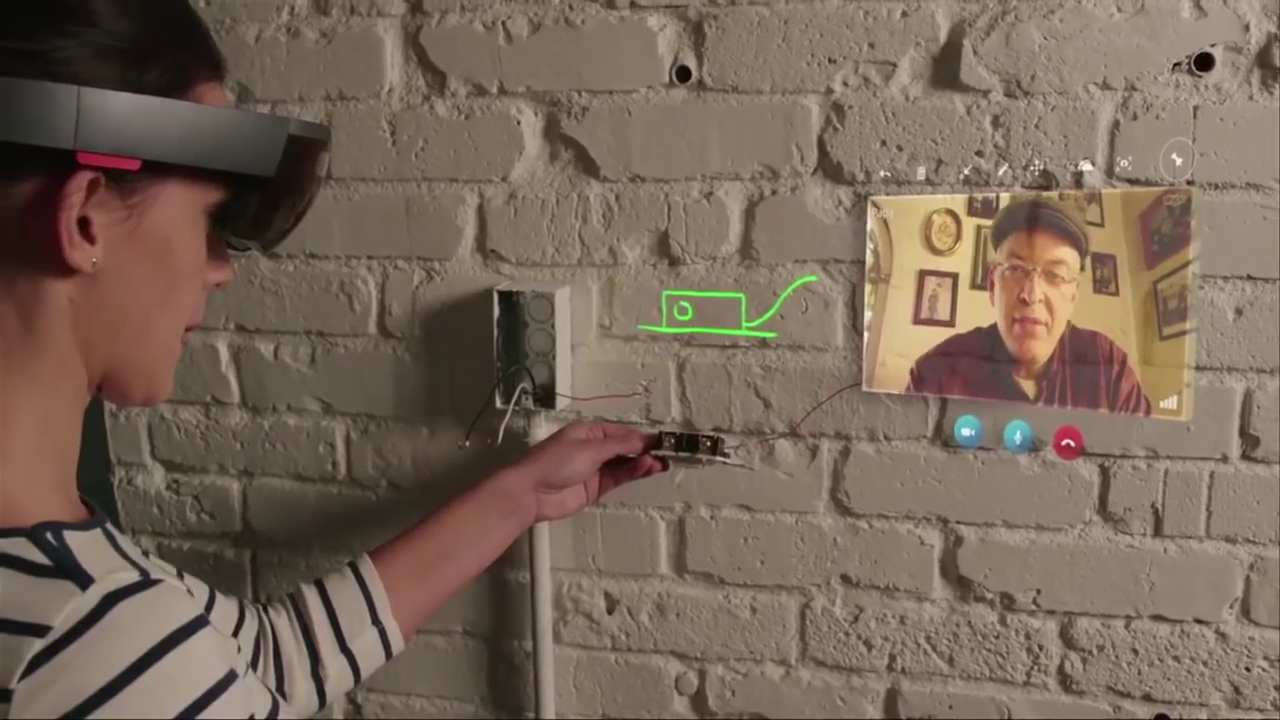
\includegraphics[width=0.4\textwidth]{\conclusion/fig/ar/hololens_fix1} &
  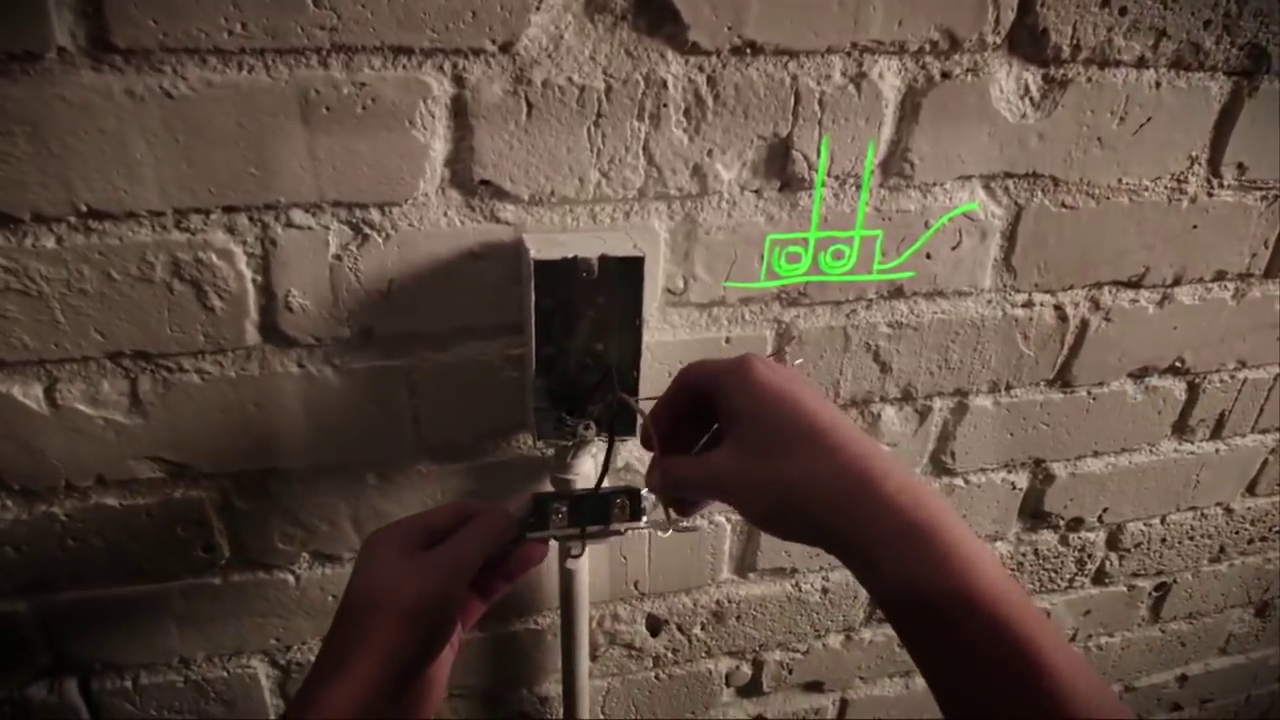
\includegraphics[width=0.4\textwidth]{\conclusion/fig/ar/hololens_fix2} \\
\multicolumn{2}{c}{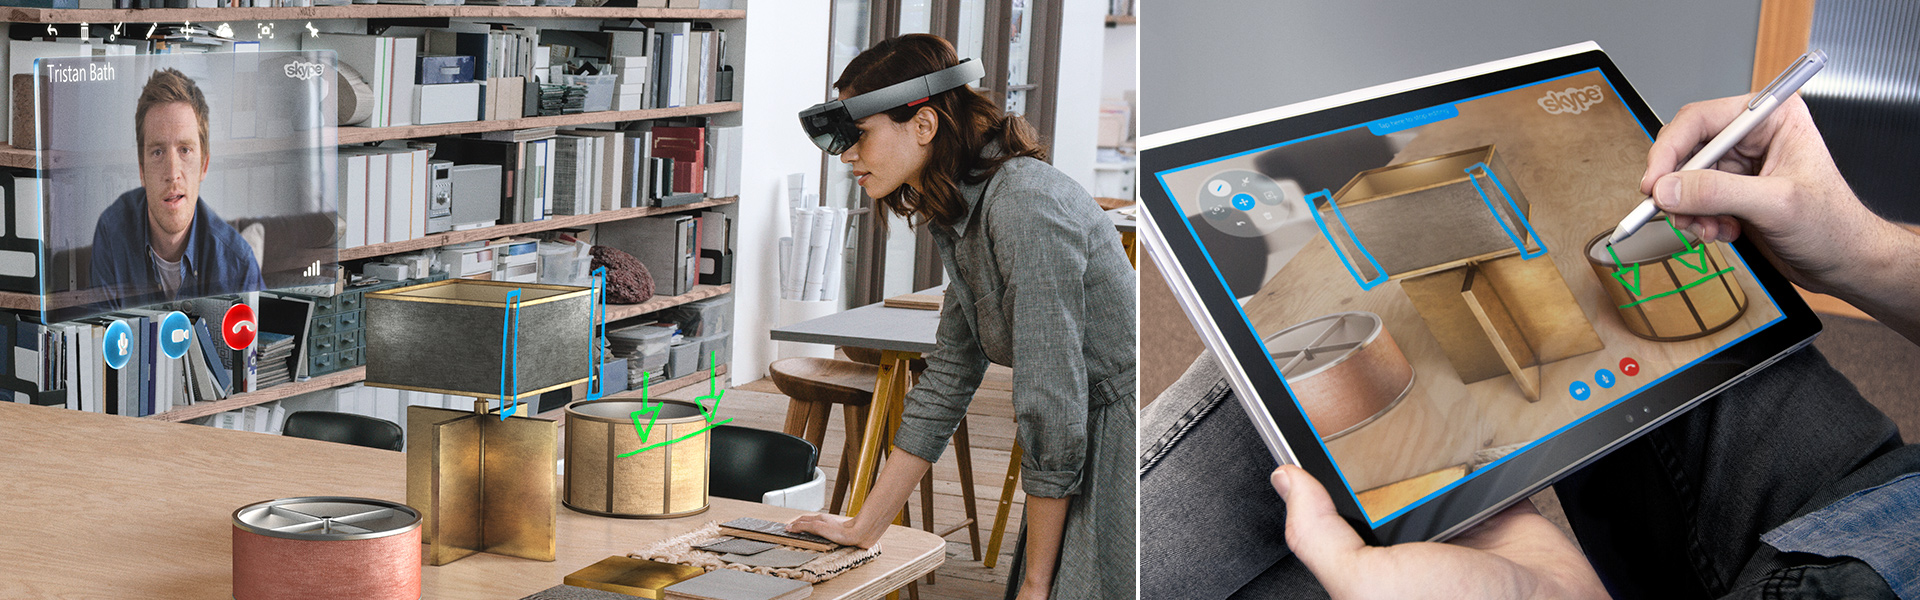
\includegraphics[width=0.82\textwidth]{\conclusion/fig/ar/hololens_skype} }
\end{tabular}
\caption{
  Microsoft's HoloLens~\cite{MicrosoftHoloLensSkype} has introduced an Augmented Reality application on providing real-time physical instructions from a remote instructor.
}
\end{figure*}

\section{Conclusion}
In this dissertation, we present video-based approaches designed for amateur users to produce and consume effective instructions from demonstrations. Using video and audio analysis techniques, our tools support recording, editing, and playback in a tutorial production process. We demonstrate results of our computer-generated tutorials from several domains, including software applications and physical activities. Our goal is to increase the quality of instructions created by tutorial authors and to support learners navigating and following the tutorials.

